\documentclass[usenames,dvipsnames,mathserif,notheorems]{beamer}

% silence annoying warnings
\usepackage{silence}
\usepackage{caption}
\WarningFilter{remreset}{The remreset package}
\usepackage{xcolor}
\usepackage{algorithm}
\usepackage{algorithmic}
\usepackage{centernot}

%% Math macros for LaTex Projects 
%% Maintainer: Aaron Mishkin <amishkin@cs.stanford.edu>
%% Original Source: Mark Schmidt (UBC CS), Ben Bloem-Reddy (UBC Stats).

%% Easy bold-face 

\def\bfA{\mathbf{A}}
\def\bfB{\mathbf{B}}
\def\bfC{\mathbf{C}}
\def\bfD{\mathbf{D}}
\def\bfE{\mathbf{E}}
\def\bfF{\mathbf{F}}
\def\bfG{\mathbf{G}}
\def\bfH{\mathbf{H}}
\def\bfI{\mathbf{I}}
\def\bfJ{\mathbf{J}}
\def\bfK{\mathbf{K}}
\def\bfL{\mathbf{L}}
\def\bfM{\mathbf{M}}
\def\bfN{\mathbf{N}}
\def\bfO{\mathbf{O}}
\def\bfP{\mathbf{P}}
\def\bfQ{\mathbf{Q}}
\def\bfR{\mathbf{R}}
\def\bfS{\mathbf{S}}
\def\bfT{\mathbf{T}}
\def\bfU{\mathbf{U}}
\def\bfV{\mathbf{V}}
\def\bfW{\mathbf{W}}
\def\bfX{\mathbf{X}}
\def\bfY{\mathbf{Y}}
\def\bfZ{\mathbf{Z}}

% bb series
\def\bbA{\mathbb{A}}
\def\bbB{\mathbb{B}}
\def\bbC{\mathbb{C}}
\def\bbD{\mathbb{D}}
\def\bbE{\mathbb{E}}
\def\bbF{\mathbb{F}}
\def\bbG{\mathbb{G}}
\def\bbH{\mathbb{H}}
\def\bbI{\mathbb{I}}
\def\bbJ{\mathbb{J}}
\def\bbK{\mathbb{K}}
\def\bbL{\mathbb{L}}
\def\bbM{\mathbb{M}}
\def\bbN{\mathbb{N}}
\def\bbO{\mathbb{O}}
\def\bbP{\mathbb{P}}
\def\bbQ{\mathbb{Q}}
\def\bbR{\mathbb{R}}
\def\bbS{\mathbb{S}}
\def\bbT{\mathbb{T}}
\def\bbU{\mathbb{U}}
\def\bbV{\mathbb{V}}
\def\bbW{\mathbb{W}}
\def\bbX{\mathbb{X}}
\def\bbY{\mathbb{Y}}
\def\bbZ{\mathbb{Z}}

% cal series
\def\calA{\mathcal{A}}
\def\calB{\mathcal{B}}
\def\calC{\mathcal{C}}
\def\calD{\mathcal{D}}
\def\calE{\mathcal{E}}
\def\calF{\mathcal{F}}
\def\calG{\mathcal{G}}
\def\calH{\mathcal{H}}
\def\calI{\mathcal{I}}
\def\calJ{\mathcal{J}}
\def\calK{\mathcal{K}}
\def\calL{\mathcal{L}}
\def\calM{\mathcal{M}}
\def\calN{\mathcal{N}}
\def\calO{\mathcal{O}}
\def\calP{\mathcal{P}}
\def\calQ{\mathcal{Q}}
\def\calR{\mathcal{R}}
\def\calS{\mathcal{S}}
\def\calT{\mathcal{T}}
\def\calU{\mathcal{U}}
\def\calV{\mathcal{V}}
\def\calW{\mathcal{W}}
\def\calX{\mathcal{X}}
\def\calY{\mathcal{Y}}
\def\calZ{\mathcal{Z}}


%% Theorem Environments %%
\usepackage{amsthm}
\usepackage{thmtools, thm-restate}
\declaretheorem{theorem}
\declaretheorem{proposition}
\declaretheorem{remark}
\declaretheorem{lemma}
\declaretheorem{definition}
\declaretheorem{assumption}
\declaretheorem{corollary}
\declaretheorem{example}

%% Floor and Ceiling %%
\usepackage{mathtools} % required for \DeclarePairedDelimeter

%% Stochastic Relations %% 

% almost sure:
\newcommand{\as}[1]{\stackrel{\text{\rm\tiny a.s.}}{#1}}
% a.s.\ equality:
\newcommand{\equas}{\stackrel{\text{\rm\tiny a.s.}}{=}}

% in distribution:
\newcommand{\dist}[1]{\stackrel{\text{\rm\tiny dist}}{#1}}
% equality in distribution:
\newcommand{\equdist}{\stackrel{\text{\rm\tiny dist}}{=}}

% independent
\newcommand{\ind}[0]{\perp \!\!\! \perp }

%% Variance, Expectation, etc %%
\newcommand{\Var}[1]{\textbf{Var}\sbr{#1}}

% ceiling and floor
\DeclarePairedDelimiter{\ceil}{\lceil}{\rceil}
\DeclarePairedDelimiter{\floor}{\lfloor}{\rfloor}
\newcommand{\argdot}{{\,\vcenter{\hbox{\tiny$\bullet$}}\,}} %generic argument dot

% absolute value
\newcommand{\abs}[1]{\left\vert #1\right\vert}

\newcommand{\seq}[1]{\rbr{#1}}

% easy bracketing:
\newcommand{\rbr}[1]{\left(#1\right)}
\newcommand{\sbr}[1]{\left[#1\right]}
\newcommand{\cbr}[1]{\left\{#1\right\}}
\newcommand{\abr}[1]{\left\langle#1\right\rangle}

% Norms
\def\norm#1{\|#1\|}
\def\biggnorm#1{\bigg\|#1\bigg\|}
% Random Variable Norms:
\def\psitwo#1{\|#1\|_{\psi_2}}
\def\psione#1{\|#1\|_{\psi_1}}

% mid
\newcommand{\biggmid}{\bigg \vert }

% argmax/argmin
\def\argmax{\mathop{\rm arg\,max}}
\def\argmin{\mathop{\rm arg\,min}}

% General Symbols
\def\half{\frac 1 2}
\newcommand{\inv}[1]{\frac{1}{#1}}
\newcommand{\halved}[1]{\frac{#1}{2}}
\newcommand{\R}{\mathbb{R}}
\newcommand{\eR}{\bar{\mathbb{R}}}

\newcommand{\into}{\rightarrow}

% Gradient Descent Symbols
\newcommand{\oracle}{\mbox{\( \calO \)}}
\newcommand{\iter}{k}

\newcommand{\Lk}{L_{\zk}}
\newcommand{\Lmax}{L_{\text{max}}}
\newcommand{\mumax}{\mu_{\text{max}}}
\newcommand{\Lmin}{L_{\text{min}}}
\newcommand{\mumin}{\mu_{\text{min}}}

% iterates
\newcommand{\y}{y}
\newcommand{\yk}{y_k}
\newcommand{\ykk}{y_{k+1}}

\newcommand{\vk}{v_k}
\newcommand{\vkk}{v_{k+1}}

\newcommand{\w}{w}
\newcommand{\wk}{w_k}
\newcommand{\wkk}{w_{k+1}}
\newcommand{\wopt}{w^*}
\newcommand{\wbar}{\bar{w}}


\newcommand{\x}{x}
\newcommand{\xk}{x_k}
\newcommand{\xkplus}{x_k^+}
\newcommand{\xkk}{x_{k+1}}
\newcommand{\xopt}{x^*}
\newcommand{\xbar}{\xbar{w}}

% noise
\newcommand{\Z}{Z}
\newcommand{\z}{z}
\newcommand{\zk}{z_{k}}
\newcommand{\zkk}{z_{k+1}}
% step-sizes
\newcommand{\tetak}{{\tilde{\eta}}_{k}}
\newcommand{\etamin}{\eta_{\text{min}}}
\newcommand{\etamax}{\eta_{\text{max}}}
\newcommand{\etak}{\eta_k}
\newcommand{\etakk}{\eta_{k+1}}

\newcommand{\betak}{\beta_{k}}
\newcommand{\betakk}{\beta_{k+1}}
\newcommand{\alphak}{\alpha_{k}}
\newcommand{\alphakk}{\alpha_{k+1}}

\newcommand{\Ek}{\bbE_{\zk}}
\newcommand{\E}{\bbE}

% functions
\newcommand{\f}{f}
\newcommand{\fj}{f_i}
\newcommand{\fopt}{f^*}
% sub-sampled functions
\newcommand{\fk}{f_{i_k}}
\newcommand{\fkk}{f_{i_{(k+1)}}}
% gradients
\newcommand{\grad}{\nabla f}
% sub-sampled gradients
\newcommand{\gradk}{\nabla f_{i_k}}
\newcommand{\gradkk}{\nabla f_{i_{(k+1)}}}

%% Weak and strong growth constants
\newcommand{\sgc}{\rho}
\newcommand{\wgc}{\alpha}
%%%%%%%%%%%%%%%%%%%%%%%%%%%%%%%%%%%%%%%%%%%%%%%%%%%%%%%%%%


%% Etc %%  

%% add numbers to align* environments.
\newcommand{\addnumber}{\addtocounter{equation}{1}\tag{\theequation}}

%%%%%%%%%

%% Group Lasso %%
\newcommand{\bi}{{i}}
\newcommand{\wi}{w_\bi}
\newcommand{\vi}{v_\bi}
\newcommand{\ci}{c_\bi}
\newcommand{\zi}{z_\bi}
\newcommand{\Xbi}{X_\bi}
\newcommand{\act}{{\calA_{\lambda}}}
\newcommand{\inact}{{\calI_{\lambda}}}
\newcommand{\tran}{{\calT_{\lambda}}}
\newcommand{\equi}{{\calE_{\lambda}}}

\newcommand{\acts}{{\calA_{\lambda}^{*}}}
\newcommand{\trans}{{\calT_{\lambda}^{*}}}

\newcommand{\wa}{w_\act}
\newcommand{\was}{w_\acts}
\newcommand{\we}{w_\equi}
\newcommand{\va}{v_\act}
\newcommand{\vas}{v_\acts}
\newcommand{\ca}{c_\act}
\newcommand{\cas}{c_\acts}
\newcommand{\ve}{v_\equi}
\newcommand{\ce}{c_\equi}
\newcommand{\Xa}{X_\act}
\newcommand{\Xas}{X_\acts}
\newcommand{\Xe}{X_\equi}

\newcommand{\wmin}{w^*}
\newcommand{\solfn}{\calW^*}

\newcommand{\Null}{\text{Null}}
\newcommand{\Row}{\text{Row}}
\newcommand{\Span}{\text{Span}}
\newcommand{\Range}{\text{Range}}

\newcommand{\Di}{\calD_{\bi}}
\newcommand{\Si}{\calN_{\bi}}
\newcommand{\Dis}{\Di^{*}}
\newcommand{\Sis}{\Ni^{*}}
\newcommand{\Ds}{\calD^{*}_\lambda}
\newcommand{\Ss}{\calN^{*}_\lambda}

\newcommand{\Ki}{K_{\bi}}
\newcommand{\Kid}{K_{\Di}}
\newcommand{\Kids}{K_{\Di^*}}
\newcommand{\Kd}{K_{\calD}}
\newcommand{\Kda}{K_{\calD \cap \act}}
\newcommand{\Kdas}{K_{\Gs}}
\newcommand{\Ka}{K_\act}

\newcommand{\Gs}{\calG^{*}_{\lambda}}

% dual parameters
\newcommand{\ri}{\rho_{\bi}}
\newcommand{\ract}{\rho_{\act}}
\newcommand{\racts}{\rho_{\acts}}
\newcommand{\rid}{\rho_{\Di}}
\newcommand{\rd}{\rho_{\calD}}
\newcommand{\rda}{\rho_{\calD \cap \act}}
\newcommand{\rdas}{\rho_{\Gs}}
\newcommand{\ra}{\rho_{\act}}
\newcommand{\rmin}{\rho^*}

\newcommand{\vmin}{v^*}
\newcommand{\diag}{\text{diag}}
\newcommand{\nnz}{\text{nnz}}

%% Plotting macros for LaTex Projects 
%% Maintainer: Aaron Mishkin <amishkin@cs.stanford.edu>


%% Tikz and PGFplots packages
\usepackage{tikz}
\usepackage{pgfplots}

% tikz and PGFplots libraries
\usepgfplotslibrary{fillbetween}
\usetikzlibrary{patterns}



%% tikz settings 
\tikzset{
    font={\fontsize{12pt}{12}\selectfont},
}

%% PGFplots settings 
\pgfplotsset{
    % version compatibility
    compat=1.5.1,
    % basic line-styles
    primary/.style={color=black, style=solid, line width=1.5pt}, 
    secondary/.style={color=red, style=solid, line width=1.5pt}, 
}


\pgfdeclarelayer{ft}
\pgfdeclarelayer{bg}
\pgfsetlayers{bg,main,ft}

\usepackage{simplebeam}
\usetheme{simplebeamer}

\usetikzlibrary{shapes, arrows}
\usetikzlibrary{decorations.pathreplacing, calligraphy}

% node styles
\tikzstyle{Input}=[minimum size=0.3cm, fill=black, line width = 0.5mm, draw=black, shape=circle, text=black]
\tikzstyle{Hidden}=[minimum size=0.3cm, fill=blue, line width = 0.5mm, draw=blue, shape=circle, text=blue]
\tikzstyle{Splits}=[inner sep=0.03cm, minimum size=0.3cm, line width = 0.3mm, draw=blue, shape=circle, text=black]
\tikzstyle{Output}=[minimum size=0.3cm, fill=white, line width = 0.5mm, draw=black, shape=circle, text=black]

% Edge styles
\tikzstyle{arrow}=[line width = 0.5mm]

% bib resources

\addbibresource[]{refs.bib}

\title{Optimal Sets and Solution Paths of ReLU Networks}
%\subtitle{}
\author{Aaron Mishkin \and Mert Pilanci}
\institute{ICML 2023}
\collaborators{
	
\includegraphics[width=0.2\linewidth]{assets/flatiron_small.jpeg}
	
\includegraphics[width=0.2\linewidth]{assets/mert.jpg}
}

\titlegraphic{
\includegraphics[width=0.4\textwidth]{assets/SUSig_2color_Stree_Left.eps}}

\newcommand{\horizontalrule}{
	{
			\vspace{-0.5em}
			\center \rule{\textwidth}{0.1em}
			\vspace{-0.2em}
		}
}

\definecolor{bad}{HTML}{eb6223}
\definecolor{good}{HTML}{9434ed}

\newcommand{\bad}[1]{\textcolor{bad}{#1}}
\newcommand{\good}[1]{\textcolor{good}{#1}}
\newcommand{\purple}[1]{\textcolor{Magenta}{#1}}

% toggle plotting tikz
\def\showtikz{}

%\logo{
\includegraphics[height=0.5cm]{assets/Block_S_2_color.eps}}

%\institute{Stanford University}
\date{}

\begin{document}

\maketitle
%% main content starts %%

\begin{frame}{The Problem}

	{
		\large \bad{Problem}: We don't understand the solution space of
		(even shallow) ReLU networks nearly as well as that of \good{GLMs}.
	}

	\pause
	\vspace{0.5em}
	\horizontalrule
	\vspace{0.5em}

	{
		\large
		Consider the Lasso:
	}

	\pause
	\vspace{0.5em}

	\begin{enumerate}
		\item \textbf{Optimal Sets}: we have an exact \good{polyhedral characterization} and simple criteria for \good{uniqueness} (general position) \citep{tibshirani2013unique}.\pause

		\item \textbf{Regularization Paths}: the (min-norm) solution path is \good{continuous} and \good{piece-wise linear} \citep{osborne2000new}.

		\item \textbf{Algorithms}: we have efficient algorithms for \good{homotopy} \citep{efron2004least} and computing \good{minimal solutions} \citep{tibshirani2013unique}.
	\end{enumerate}

\end{frame}

\begin{frame}{Challenges from Non-Convexity}
	\begin{center}
		\Large
		Non-convexity makes extensions beyond GLMs \bad{hard}!
	\end{center}

	\begin{figure}[]
		\centering
		\ifdefined\showtikz
			%! TEX root = ../../main.tex
%% Illustration of step-sizes bound from Armijo line-search. 

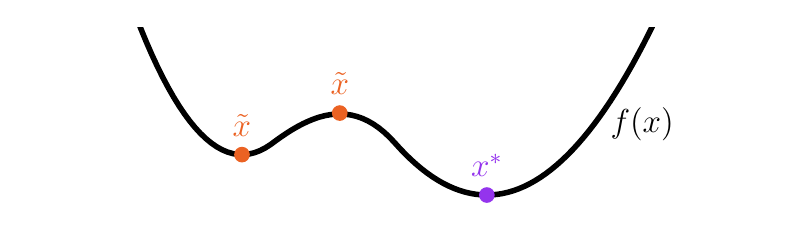
\begin{tikzpicture}[scale=1,
		declare function={
				objective(\x)=      (\x<=-1) * (2*\x*\x + 6*\x + 4)    +
				and(\x>-1, \x<=1) * (\x + 5 - pow(\x,3) - 5*\x*\x) / 4 +
				(\x>1) * (\x*\x - 5*\x + 4);
			}
	]
	\begin{axis}[
			width=0.9\textwidth,
			height=4cm,
			axis x line=none, axis y line=none,
			ymin=-3.25, ymax=5, ytick={-5,...,5}, ylabel=$y$,
			xmin=-5, xmax=7, xtick={-5,...,7}, xlabel=$x$,
		]

		\addplot[name path=function, domain=-3.5:5.23, samples=100, line width=2pt]{objective(x)};

		\node[label={[text=good]90:$x^*$},circle,fill=good,inner sep=2pt] at (axis cs:2.5,-2.25) {};
		\node[label={[text=bad]90:$\tilde x$},circle,fill=bad,inner sep=2pt] at (axis cs:0.09717,1.3) {};
		\node[label={[text=bad]90:$\tilde x$},circle,fill=bad,inner sep=2pt] at (axis cs:-1.5,-0.5) {};

		\node[label={0:$f(x)$}] at (axis cs:4.2,0.8) {};
	\end{axis}
\end{tikzpicture}


		\else
			\Huge Non-Convex Figure
		\fi
	\end{figure}

	\pause
	\begin{itemize}
		\item \textbf{Optimality Conditions}: Stationarity \( \centernot \implies \) optimality.
		      We have no global optimality criteria and no certificates.

		      \vspace{1em}

		      \pause
		\item \textbf{Mathematical Tools}: Our perspective completely changes
		      to reasoning about saddles, Clarke stationary points, etc.
		      \vspace{1em}

		      \pause

		\item \textbf{Unintuitive Phenomena}: surprising things happen even
		      with toy neural networks\ldots

	\end{itemize}

\end{frame}

\begin{frame}{Example: Discontinuous Paths}
	Consider training a toy network:
	\[
		\min_{w} \, ((w x_1)_+ - y_1)^2 + ((w x_2)_+ - y_2)^2 + \lambda |w|.
	\]

	\begin{center}
		%! TEX root = ../../main.tex

%% Illustration of cone decomposition. 

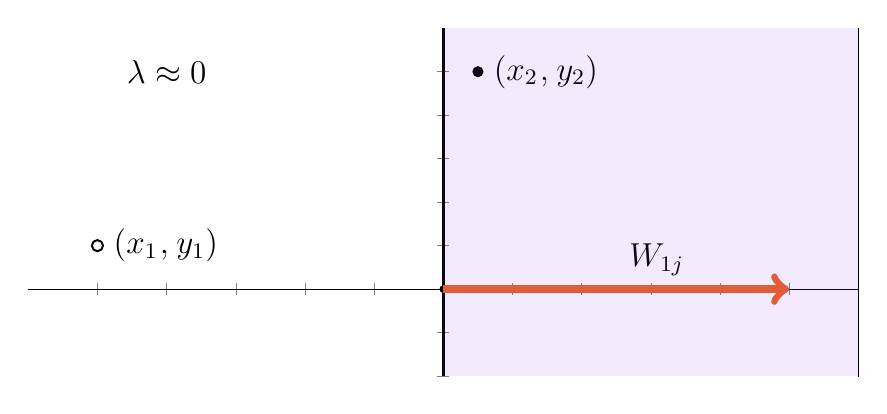
\begin{tikzpicture}[scale=1,
		declare function={
				cone_1(\x)= 10*\x;
				cone_2(\x)= -\x;
				cone_3(\x)= -4*\x;
				bounds(\x)= \x - 10;
			}
	]
	\begin{axis}[width=\linewidth, height=6cm,
			axis lines=center, yticklabels={,,}, xticklabels={,,},
			ymin=-2, ymax=6, ytick={-2,...,5}, ylabel=$$, x axis line style={-},
				xmin=-6, xmax=6, xtick={-5,...,5}, xlabel=$$, y axis line style={-},
		]

		\draw [name path=cone_1, solid, line width=1pt] (axis cs:0,-2) -- (axis cs:0,6);
		\draw [name path=bounds, line width=0pt] (axis cs:6,-2) -- (axis cs:6,6);
		\tikzfillbetween[of=cone_1 and bounds, on layer=ft]{good, opacity=0.1};

		%% point labels
		% origin point
		\node[circle, fill, inner sep=1pt] at (axis cs:0,0) {};

		% active examples 
		\node[label=right:$(x_1\!\mathbin{,} y_1)$, circle, draw, line width=0.25mm, inner sep=0.5mm] at (axis cs:-5,1) {};
		\node[label=right:$(x_2\!\mathbin{,} y_2)$, circle, fill, inner sep=0.5mm] at (axis cs:0.5,5) {};


		% lines
		\draw [->, draw=bad, line width = 1mm] (axis cs:0,0) -- (axis cs:5,0) node[midway,above right] {$W_{1j}$};

        \node[] at (axis cs:-4,5) { $ \lambda \approx 0$ };
	\end{axis}

\end{tikzpicture}%

	\end{center}

	\begin{center}
		\Large
		\textcolor{white}{Goal: New insights via convexification.}
	\end{center}

\end{frame}

\begin{frame}{Example: Discontinuous Paths}
	Consider training a toy network:
	\[
		\min_{w} \, ((w x_1)_+ - y_1)^2 + ((w x_2)_+ - y_2)^2 + \lambda |w|.
	\]

	\begin{center}
		%! TEX root = ../../main.tex

%% Illustration of cone decomposition. 

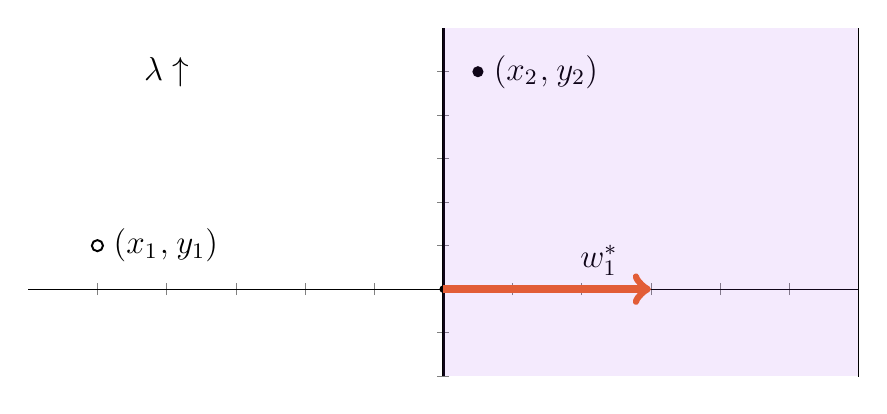
\begin{tikzpicture}[scale=1,
		declare function={
				cone_1(\x)= 10*\x;
				cone_2(\x)= -\x;
				cone_3(\x)= -4*\x;
				bounds(\x)= \x - 10;
			}
	]
	\begin{axis}[width=\linewidth, height=6cm,
			axis lines=center, yticklabels={,,}, xticklabels={,,},
			ymin=-2, ymax=6, ytick={-2,...,5}, ylabel=$$, x axis line style={-},
				xmin=-6, xmax=6, xtick={-5,...,5}, xlabel=$$, y axis line style={-},
		]

		\draw [name path=cone_1, solid, line width=1pt] (axis cs:0,-2) -- (axis cs:0,6);
		\draw [name path=bounds, line width=0pt] (axis cs:6,-2) -- (axis cs:6,6);
		\tikzfillbetween[of=cone_1 and bounds, on layer=ft]{good, opacity=0.1};

		%% point labels
		% origin point
		\node[circle, fill, inner sep=1pt] at (axis cs:0,0) {};

		% active examples 
		\node[label=right:$(x_1\!\mathbin{,} y_1)$, circle, draw, line width=0.25mm, inner sep=0.5mm] at (axis cs:-5,1) {};
		\node[label=right:$(x_2\!\mathbin{,} y_2)$, circle, fill, inner sep=0.5mm] at (axis cs:0.5,5) {};


		% lines
		\draw [->, draw=bad, line width = 1mm] (axis cs:0,0) -- (axis cs:3,0) node[near end,above] {$w^*_{1}$};

        \node[] at (axis cs:-4,5) { $ \lambda \uparrow $ };
	\end{axis}

\end{tikzpicture}%

	\end{center}

	\begin{center}
		\Large
		\textcolor{white}{Goal: New insights via convexification.}
	\end{center}


\end{frame}

\begin{frame}{Example: Discontinuous Paths}
	Consider training a toy network:
	\[
		\min_{w} \, ((w x_1)_+ - y_1)^2 + ((w x_2)_+ - y_2)^2 + \lambda |w|.
	\]

	\begin{center}
		%! TEX root = ../../main.tex

%% Illustration of cone decomposition. 

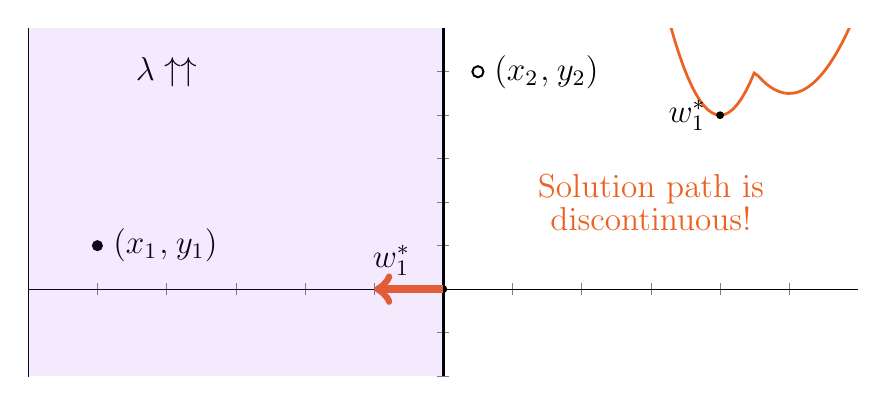
\begin{tikzpicture}[scale=1,
		declare function={
				loss(\x)= (4*(\x - 4)^2 + 4)*(x<=4.5) + (2*(\x - 5)^2 + 4.5)*(x>4.5);
			}
	]
	\begin{axis}[width=\linewidth, height=6cm,
			axis lines=center, yticklabels={,,}, xticklabels={,,},
			ymin=-2, ymax=6, ytick={-2,...,5}, ylabel=$$, x axis line style={-},
				xmin=-6, xmax=6, xtick={-5,...,5}, xlabel=$$, y axis line style={-},
		]
		\addplot[name path=loss, domain=-6:6, samples=200, line width=1pt, color=bad]{loss(x)};
		\node[label=left:$w_1^*$, circle, fill, inner sep=1pt] at (axis cs:4,4) {};

		\draw [name path=cone_1, solid, line width=1pt] (axis cs:0,-2) -- (axis cs:0,6);
		\draw [name path=bounds, line width=0pt] (axis cs:-6,-2) -- (axis cs:-6,6);
		\tikzfillbetween[of=cone_1 and bounds, on layer=ft]{good, opacity=0.1};

		%% point labels
		% origin point
		\node[circle, fill, inner sep=1pt] at (axis cs:0,0) {};

		% active examples 
		\node[label=right:$(x_1\!\mathbin{,} y_1)$, circle, fill, inner sep=0.5mm] at (axis cs:-5,1) {};
		\node[label=right:$(x_2\!\mathbin{,} y_2)$, circle, draw, line width=0.25mm, inner sep=0.5mm] at (axis cs:0.5,5) {};


		% lines
		\draw [->, draw=bad, line width = 1mm] (axis cs:0,0) -- (axis cs:-1,0) node[near end,above] {$w^*_{1}$};

		\node[] at (axis cs:-4,5) { $ \lambda \uparrow \uparrow$ };
    \node[text width=13em, text centered] at (axis cs:3,2) { \bad{Solution path} \bad{is discontinuous!} };
	\end{axis}

\end{tikzpicture}%

	\end{center}

	\pause

	\begin{center}
		\Large
		\good{Goal}: New insights via convexification.
	\end{center}

\end{frame}

\begin{frame}{Our Contributions}

	{
		\large \good{Our Contribution}: leverage convex reformulations
		of ReLU networks \citep{pilanci2020convex} as an analytical tool.
	}

	\pause
	\vspace{0.5em}
	\horizontalrule
	\vspace{0.5em}

	\begin{enumerate}
		\item \textbf{Optimal Sets}: we characterize all optima of the
		      non-convex training objective.\pause
		      \vspace{0.5em}

		\item \textbf{Uniqueness}: we develop simple criteria for ReLU networks
		      to admit unique solutions up permutation/split symmetries. \pause
		      \vspace{0.5em}

		\item \textbf{Optimal Pruning}: we leverage our theory to give a
		      poly-time procedure for computing minimal ReLU networks.
	\end{enumerate}

\end{frame}


\setbeamercolor{background canvas}{bg=LightCyan}
\begin{frame}{}
	\begin{center}
		\huge I. Background on Convex Reformulations
	\end{center}
\end{frame}
\setbeamercolor{background canvas}{bg=white}

\begin{frame}{Convex Reformulations: Flavor of Results}
	\large

	\textbf{Basic Idea}: We start with a \bad{non-convex} optimization problem and derive
	an equivalent \good{convex} program.

	\pause
	\vspace{2em}

	\textbf{Equivalent} means:
	\vspace{0.5em}
	\begin{itemize}
		\item The global minima have the same values: \( p^* = q^* \)
		      \vspace{0.5em}
		\item We can map a solution \( u^* \) for one problem into a solution
		      \( v^* \) for the other.
		      \vspace{0.5em}
	\end{itemize}

\end{frame}


\begin{frame}{Convex Reformulations: Two-Layer ReLU Networks}

	{\large \bad{Non-Convex Problem}}
	\[
		\min_{W_1, w_2} \underbrace{\half \norm{\sum_{j=1}^m (X W_{1j})_+ w_{2j} - y}_2^2}_{\text{Squared Error}}
		+ \underbrace{\lambda \sum_{j=1}^m \norm{W_{1j}}_2^2 + |w_{2j}|^2}_{\text{Weight Decay}},
	\]
	where \( \rbr{x}_+ = \max\cbr{x, 0} \) is the ReLU activation.
	\pause

	\begin{figure}[]
		\centering
		\ifdefined\showtikz
			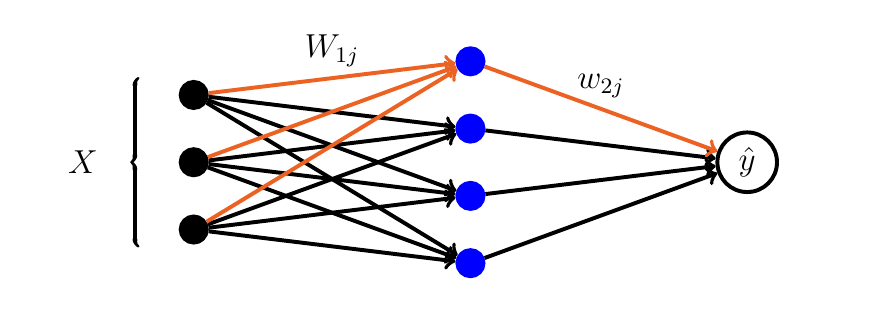
\begin{tikzpicture}[scale=1,
	]
	\begin{axis}[width=\linewidth, height=5cm,
			axis lines=none,  % don't print axis lines
			yticklabels={,,}, xticklabels={,,},
			ymin=0, ymax=8, y axis line style={-},
			xmin=0, xmax=15, x axis line style={-},
		]
		\node [] (input) at (axis cs:1,4) {$X$};
		\node [Input] (input1) at (axis cs:3,2) {};
		\node [Input] (input2) at (axis cs:3,4) {};
		\node [Input] (input3) at (axis cs:3,6) {};

		\draw [decorate, line width = 0.6mm,
			decoration = {calligraphic brace}] (axis cs:2,1.5) --  (axis cs:2,6.5);

		\node [Hidden] (hidden1) at (axis cs:8,1) {};
		\node [Hidden] (hidden2) at (axis cs:8,3) {};
		\node [Hidden] (hidden3) at (axis cs:8,5) {};
		\node [Hidden] (hidden4) at (axis cs:8,7) {};

		\draw [->, style=arrow, draw=black] (input1) -- (hidden1);
		\draw [->, style=arrow, draw=black] (input2) -- (hidden1);
		\draw [->, style=arrow, draw=black] (input3) -- (hidden1);

		\draw [->, style=arrow, draw=black] (input1) -- (hidden2);
		\draw [->, style=arrow, draw=black] (input2) -- (hidden2);
		\draw [->, style=arrow, draw=black] (input3) -- (hidden2);

		\draw [->, style=arrow, draw=black] (input1) -- (hidden3);
		\draw [->, style=arrow, draw=black] (input2) -- (hidden3);
		\draw [->, style=arrow, draw=black] (input3) -- (hidden3);

		\draw [->, style=arrow, draw=bad] (input1) -- (hidden4);
		\draw [->, style=arrow, draw=bad] (input2) -- (hidden4);
		\draw [->, style=arrow, draw=bad] (input3) -- (hidden4) node[pos=0.5,above] {$W_{1j}$};

		\node [Output] (output) at (axis cs:13,4) {$\hat y$};

		\draw [->, style=arrow, draw=black] (hidden1) -- (output);
		\draw [->, style=arrow, draw=black] (hidden2) -- (output);
		\draw [->, style=arrow, draw=black] (hidden3) -- (output);
		\draw [->, style=arrow, draw=bad] (hidden4) -- (output) node[pos=0.5,above] {$w_{2j}$};
	\end{axis}

\end{tikzpicture}%

%\begin{tikzpicture}[scale=1,
%    ]
%    \begin{axis}[width=1.1\linewidth, height=5cm,
%            axis lines=none,  % don't print axis lines
%            yticklabels={,,}, xticklabels={,,},
%            ymin=-0.2, ymax=10.2, x axis line style={-},
%            xmin=-0.2, xmax=20.2, y axis line style={-},
%        ]

%        \filldraw[color=blue!60, fill=blue!5, line width=0.4mm](axis cs:0,5.8) rectangle (axis cs:20, 10);
%        \filldraw[color=red!60, fill=red!5, line width=0.4mm](axis cs:0,0) rectangle (axis cs:20, 4.2);

%        % non-convex models
%        \filldraw[line width=0.4mm, fill=white](axis cs:1,1) rectangle (axis cs:8, 3.2) node[pos=.5] {NC-GReLU};
%        \filldraw[line width=0.4mm, fill=white](axis cs:12,1) rectangle (axis cs:19, 3.2) node[pos=.5] {NC-ReLU};

%        % convex models
%        \filldraw[line width=0.4mm, fill=white](axis cs:1,6.8) rectangle (axis cs:8, 9) node[pos=.5] {C-GReLU};
%        \filldraw[line width=0.4mm, fill=white](axis cs:12,6.8) rectangle (axis cs:19, 9) node[pos=.5] {C-ReLU};

%        \draw [<->, solid, draw=black, line width = 0.6mm] (axis cs:4.5,3.2) -- (axis cs:4.5,6.8) node[right, pos=0.5] {\small Sol. Map};

%        \draw [<->, solid, draw=black, line width = 0.6mm] (axis cs:15.5,3.2) -- (axis cs:15.5,6.8)  node[right, pos=0.5] {\small Sol. Map};

%        \draw [<-, solid, draw=black, line width = 0.6mm] (axis cs:6,9) -- [bend left=15] (axis cs:14, 9);

%        \draw [->, solid, draw=orange, line width = 0.6mm] (axis cs:8,7.9) -- (axis cs:12,7.9);
%        \node[align=center] at (axis cs:10.1, 7.8) {\small Cone\\ \small Decomp.};
%    \end{axis}

%\end{tikzpicture}%


		\else
			\Huge Neural Network Figure
		\fi
	\end{figure}

\end{frame}


\begin{frame}{Aside: ReLU Activation Patterns}

	Each ReLU neuron is active on a half-space:

	\pause

	\begin{figure}[]
		\centering
		\ifdefined\showtikz
			%! TEX root = ../../main.tex

%% Illustration of cone decomposition. 

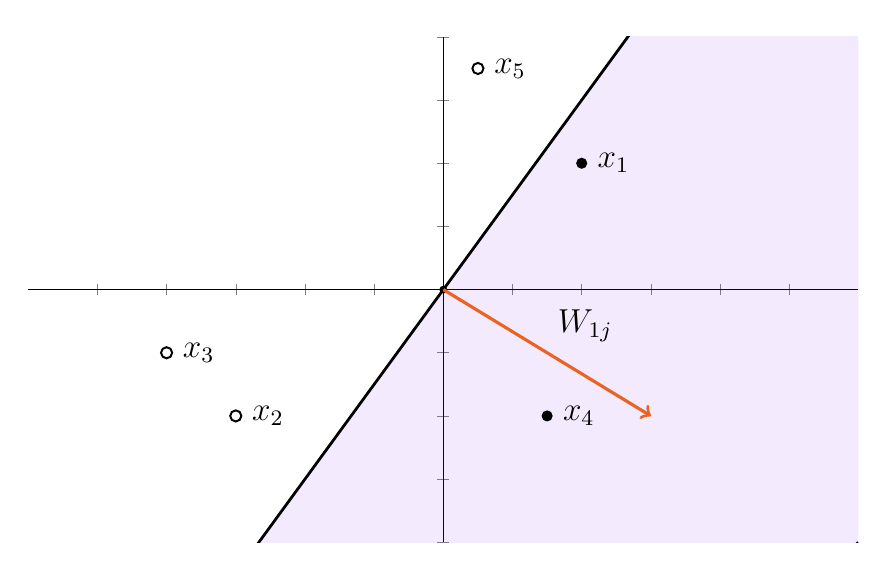
\begin{tikzpicture}[scale=1,
		declare function={
				cone_1(\x)= 3*\x/2;
				cone_2(\x)= -\x;
				cone_3(\x)= -4*\x;
				bounds(\x)= \x - 10;
			}
	]
	\begin{axis}[width=\linewidth, height=8cm,
			axis lines=center, yticklabels={,,}, xticklabels={,,},
			ymin=-4, ymax=4, ytick={-5,...,5}, ylabel=$$, x axis line style={-},
				xmin=-6, xmax=6, xtick={-5,...,5}, xlabel=$$, y axis line style={-},
		]
		\addplot[name path=cone_1, domain=-6:6, samples=100, line width=1pt]{cone_1(x)};
		\addplot[name path=bounds, domain=-6:6, samples=100, line width=1pt]{bounds(x)};

		% add color fill to both cones.

		\addplot fill between[
				of = cone_1 and bounds,
				%split, % calculate segment
				every even segment/.style = {fill=good, fill opacity=0.1},
			];

		%% point labels
		% origin point
		\node[circle, fill, inner sep=1pt] at (axis cs:0,0) {};

		% active examples 
		\node[label=right:$x_1$, circle, fill, inner sep=0.5mm] at (axis cs:2,2) {};
		\node[label=right:$x_4$, circle, fill, inner sep=0.5mm] at (axis cs:1.5,-2) {};

		% inactive examples 
		\node[label=right:$x_2$, circle, line width=0.25mm, draw=black, inner sep=0.5mm] at (axis cs:-3,-2) {};
		\node[label=right:$x_3$, circle, line width=0.25mm, draw=black, inner sep=0.5mm] at (axis cs:-4,-1) {};
		\node[label=right:$x_5$, circle, line width=0.25mm, draw=black, inner sep=0.5mm] at (axis cs:0.5,3.5) {};


		% lines
		\draw [->, draw=bad, line width = 0.4mm] (axis cs:0,0) -- (axis cs:3,-2) node[midway,above right] {$W_{1j}$};
		%\draw [->, draw=red, line width = 0.4mm] (axis cs:2,-2) -- (axis cs:3,-1) node[midway,below right] {$S_{22} \cdot x_2$};
		%\draw [->, draw=red, line width = 0.4mm] (axis cs:0.5,-2) -- (axis cs:-2.5,-2.75) node[pos=0.9,below right] {$S_{33} \cdot x_3$};
	\end{axis}

\end{tikzpicture}%

		\else
			\Huge activation pattern figure
		\fi
	\end{figure}

	\phantom{
		\textbf{Activation Pattern} satisfies \( D_j X W_{1j} = \rbr{X W_{1j}}_+ \)
	}

\end{frame}

\begin{frame}{Aside: ReLU Activation Patterns}

	Each ReLU neuron is active on a half-space:

	\begin{figure}[]
		\centering
		\ifdefined\showtikz
			%! TEX root = ../../main.tex

%% Illustration of cone decomposition. 

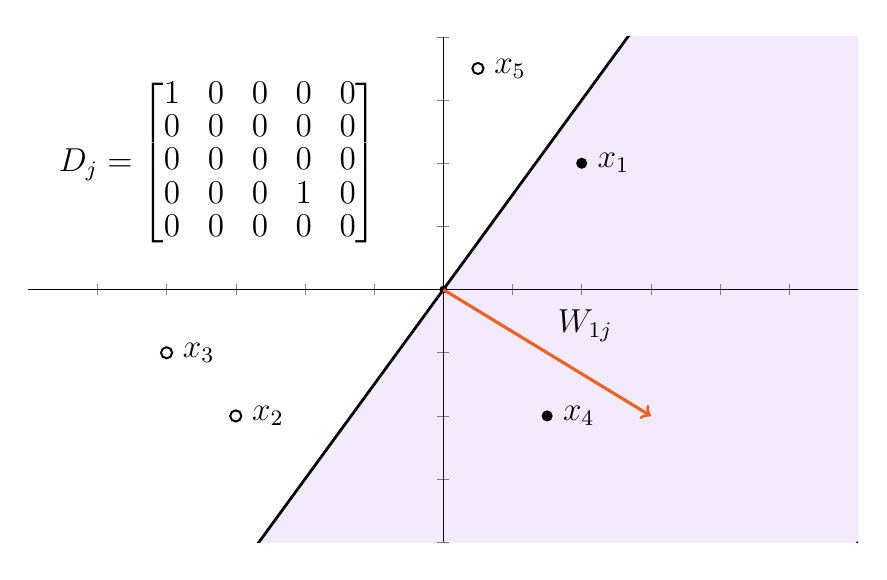
\begin{tikzpicture}[scale=1,
		declare function={
				cone_1(\x)= 3*\x/2;
				cone_2(\x)= -\x;
				cone_3(\x)= -4*\x;
				bounds(\x)= \x - 10;
			}
	]
	\begin{axis}[width=\linewidth, height=8cm,
			axis lines=center, yticklabels={,,}, xticklabels={,,},
			ymin=-4, ymax=4, ytick={-5,...,5}, ylabel=$$, x axis line style={-},
				xmin=-6, xmax=6, xtick={-5,...,5}, xlabel=$$, y axis line style={-},
		]
		\addplot[name path=cone_1, domain=-6:6, samples=100, line width=1pt]{cone_1(x)};
		\addplot[name path=bounds, domain=-6:6, samples=100, line width=1pt]{bounds(x)};

		% add color fill to both cones.

		\addplot fill between[
				of = cone_1 and bounds,
				%split, % calculate segment
				every even segment/.style = {fill=good, fill opacity=0.1},
			];

		%% point labels
		% origin point
		\node[circle, fill, inner sep=1pt] at (axis cs:0,0) {};

		% active examples 
		\node[label=right:$x_1$, circle, fill, inner sep=0.5mm] at (axis cs:2,2) {};
		\node[label=right:$x_4$, circle, fill, inner sep=0.5mm] at (axis cs:1.5,-2) {};

		% inactive examples 
		\node[label=right:$x_2$, circle, line width=0.25mm, draw=black, inner sep=0.5mm] at (axis cs:-3,-2) {};
		\node[label=right:$x_3$, circle, line width=0.25mm, draw=black, inner sep=0.5mm] at (axis cs:-4,-1) {};
		\node[label=right:$x_5$, circle, line width=0.25mm, draw=black, inner sep=0.5mm] at (axis cs:0.5,3.5) {};


		% activation pattern
		\node[] at (axis cs:-3.25,2) {
			$D_j = \begin{bmatrix}
					1 & 0 & 0 & 0 & 0 \\
					0 & 0 & 0 & 0 & 0 \\
					0 & 0 & 0 & 0 & 0 \\
					0 & 0 & 0 & 1 & 0 \\
					0 & 0 & 0 & 0 & 0 \\
				\end{bmatrix}
			$};

		% lines
		\draw [->, draw=bad, line width = 0.4mm] (axis cs:0,0) -- (axis cs:3,-2) node[midway,above right] {$W_{1j}$};
		%\draw [->, draw=red, line width = 0.4mm] (axis cs:2,-2) -- (axis cs:3,-1) node[midway,below right] {$S_{22} \cdot x_2$};
		%\draw [->, draw=red, line width = 0.4mm] (axis cs:0.5,-2) -- (axis cs:-2.5,-2.75) node[pos=0.9,below right] {$S_{33} \cdot x_3$};
	\end{axis}

\end{tikzpicture}%

		\else
			\Huge activation pattern figure
		\fi
	\end{figure}

	\pause
	\textbf{Activation Pattern} satisfies \( D_j X W_{1j} = \rbr{X W_{1j}}_+ \)

\end{frame}

\begin{frame}{Aside: ReLU Activation Patterns}

	Each ReLU neuron is active on a half-space:

	\begin{figure}[]
		\centering
		\ifdefined\showtikz
			%! TEX root = ../../main.tex

%% Illustration of cone decomposition. 

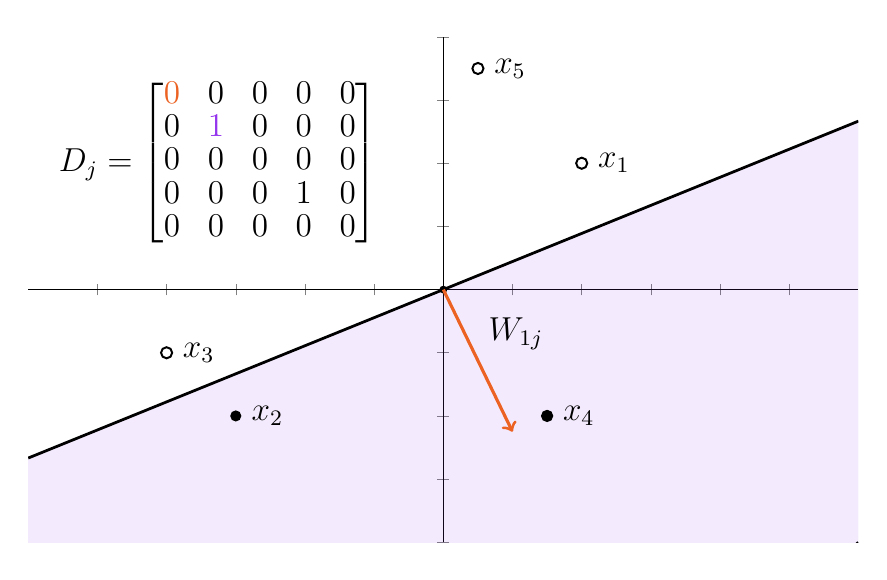
\begin{tikzpicture}[scale=1,
		declare function={
				cone_1(\x)= \x/2.25;
				cone_2(\x)= -\x;
				cone_3(\x)= -4*\x;
				bounds(\x)= \x - 10;
			}
	]
	\begin{axis}[width=\linewidth, height=8cm,
			axis lines=center, yticklabels={,,}, xticklabels={,,},
			ymin=-4, ymax=4, ytick={-5,...,5}, ylabel=$$, x axis line style={-},
				xmin=-6, xmax=6, xtick={-5,...,5}, xlabel=$$, y axis line style={-},
		]
		\addplot[name path=cone_1, domain=-6:6, samples=100, line width=1pt]{cone_1(x)};
		\addplot[name path=bounds, domain=-6:6, samples=100, line width=1pt]{bounds(x)};

		% add color fill to both cones.

		\addplot fill between[
				of = cone_1 and bounds,
				%split, % calculate segment
				every even segment/.style = {fill=good, fill opacity=0.1},
			];

		%% point labels
		% origin point
		\node[circle, fill, inner sep=1pt] at (axis cs:0,0) {};

		% active examples 
		\node[label=right:$x_1$, circle, line width=0.25mm, draw=black, inner sep=0.5mm] at (axis cs:2,2) {};
		\node[label=right:$x_4$, circle, fill, draw=black, inner sep=0.5mm] at (axis cs:1.5,-2) {};

		% inactive examples 
		\node[label=right:$x_2$, circle, fill, inner sep=0.5mm] at (axis cs:-3,-2) {};
		\node[label=right:$x_3$, circle, line width=0.25mm, draw=black, inner sep=0.5mm] at (axis cs:-4,-1) {};
		\node[label=right:$x_5$, circle, line width=0.25mm, draw=black, inner sep=0.5mm] at (axis cs:0.5,3.5) {};


		% activation pattern
		\node[] at (axis cs:-3.25,2) {
			$D_j = \begin{bmatrix}
					\bad{0} & 0        & 0 & 0 & 0 \\
					0       & \good{1} & 0 & 0 & 0 \\
					0       & 0        & 0 & 0 & 0 \\
					0       & 0        & 0 & 1 & 0 \\
					0       & 0        & 0 & 0 & 0 \\
				\end{bmatrix}
			$};

		% lines
		\draw [->, draw=bad, line width = 0.4mm] (axis cs:0,0) -- (axis cs:1,-2.25) node[midway,above right] {$W_{1j}$};

	\end{axis}

\end{tikzpicture}%

		\else
			\Huge activation pattern figure
		\fi
	\end{figure}


	\textbf{Activation Pattern} satisfies \( D_j X W_{1j} = \rbr{X W_{1j}}_+ \)

\end{frame}


\begin{frame}{Convex Reformulations: Convex Problem}

	{\large \good{Convex Reformulation}} \citep{pilanci2020convex}
	\[
		\begin{aligned}
			\min_{v, w} & \half \norm{\sum_{j=1}^p D_j X (v_j - w_j) - y}_2^2 +
			\lambda \sum_{j=1}^p \norm{v_j}_2 + \norm{w_j}_2                    \\
			            & \hspace{0.2em} \text{s.t. }
			v_j, w_j \in \calK_j := \cbr{w : (2D_j - I) X w \geq 0},
		\end{aligned}
	\]
	where \( D_j = \text{diag}[\mathbbm{1}(X g_j \geq 0)] \).
	\pause

	\begin{figure}[]
		\centering
		\ifdefined\showtikz
			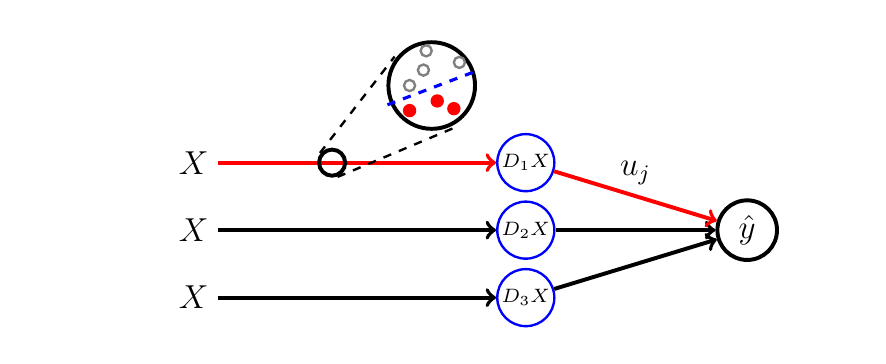
\begin{tikzpicture}[scale=1,
	]
	\begin{axis}[width=\linewidth, height=5.5cm,
			axis lines=none,  % don't print axis lines
			yticklabels={,,}, xticklabels={,,},
			ymin=0, ymax=8, y axis line style={-},
			xmin=0, xmax=15, x axis line style={-},
		]
		\node [] (input1) at (axis cs:3,1) {$X$};
		\node [] (input2) at (axis cs:3,2.75) {$X$};
		\node [] (input3) at (axis cs:3,4.5) {$X$};

        \node [Splits] (hidden1) at (axis cs:9,1) {\scriptsize $D_3 X$};
		\node [Splits] (hidden2) at (axis cs:9,2.75) {\scriptsize $D_2 X$};
		\node [Splits] (hidden3) at (axis cs:9,4.5) {\scriptsize $D_1 X$};

		\draw [->, style=arrow, draw=black] (input1) -- (hidden1);

		\draw [->, style=arrow, draw=black] (input2) -- (hidden2);

		\draw [->, style=arrow, draw=red] (input3) -- (hidden3);

		\node [Output] (output) at (axis cs:13,2.75) {$\hat y$};

		\draw [->, style=arrow, draw=black] (hidden1) -- (output);
		\draw [->, style=arrow, draw=black] (hidden2) -- (output);
		\draw [->, style=arrow, draw=red] (hidden3) -- (output) node[pos=0.5,above] {$u_j$};

		\draw [draw=black, line width=0.3mm, dashed] (axis cs:5.6, 4.13) -- (axis cs:7.7,5.4);
		\draw [draw=black, line width=0.3mm, dashed] (axis cs:5.28, 4.75) -- (axis cs:6.63,7.25);

		\node [draw=black, minimum size=0.3cm, shape=circle, solid, line width=0.5mm] (examine) at (axis cs:5.5,4.5) {};
		\node [draw=black, minimum size=1.1cm, shape=circle, solid, line width=0.5mm] (closeup) at (axis cs:7.3,6.5) {};

		\node [fill=white, draw=gray, line width=0.3mm, inner sep=0.05cm, shape=circle] at (axis cs:7.8,7.1) {};
		\node [fill=white, draw=gray, line width=0.3mm, inner sep=0.05cm, shape=circle] at (axis cs:7.15,6.9) {};
		\node [fill=white, draw=gray, line width=0.3mm, inner sep=0.05cm, shape=circle] at (axis cs:7.2,7.4) {};
		\node [fill=white, draw=gray, line width=0.3mm, inner sep=0.05cm, shape=circle] at (axis cs:6.9,6.5) {};

		\draw [draw=Blue, dashed, line width=0.4mm] (axis cs:6.5,6.) -- (axis cs:8.15,6.9);

		\node [fill=Red, inner sep=0.06cm, shape=circle] at (axis cs:6.9,5.85) {};
		\node [fill=Red, inner sep=0.06cm, shape=circle] at (axis cs:7.4,6.1) {};
		\node [fill=Red, inner sep=0.06cm, shape=circle] at (axis cs:7.7,5.9) {};

	\end{axis}

\end{tikzpicture}%

%\begin{tikzpicture}[scale=1,
%    ]
%    \begin{axis}[width=1.1\linewidth, height=5cm,
%            axis lines=none,  % don't print axis lines
%            yticklabels={,,}, xticklabels={,,},
%            ymin=-0.2, ymax=10.2, x axis line style={-},
%            xmin=-0.2, xmax=20.2, y axis line style={-},
%        ]

%        \filldraw[color=blue!60, fill=blue!5, line width=0.4mm](axis cs:0,5.8) rectangle (axis cs:20, 10);
%        \filldraw[color=red!60, fill=red!5, line width=0.4mm](axis cs:0,0) rectangle (axis cs:20, 4.2);

%        % non-convex models
%        \filldraw[line width=0.4mm, fill=white](axis cs:1,1) rectangle (axis cs:8, 3.2) node[pos=.5] {NC-GReLU};
%        \filldraw[line width=0.4mm, fill=white](axis cs:12,1) rectangle (axis cs:19, 3.2) node[pos=.5] {NC-ReLU};

%        % convex models
%        \filldraw[line width=0.4mm, fill=white](axis cs:1,6.8) rectangle (axis cs:8, 9) node[pos=.5] {C-GReLU};
%        \filldraw[line width=0.4mm, fill=white](axis cs:12,6.8) rectangle (axis cs:19, 9) node[pos=.5] {C-ReLU};

%        \draw [<->, solid, draw=black, line width = 0.6mm] (axis cs:4.5,3.2) -- (axis cs:4.5,6.8) node[right, pos=0.5] {\small Sol. Map};

%        \draw [<->, solid, draw=black, line width = 0.6mm] (axis cs:15.5,3.2) -- (axis cs:15.5,6.8)  node[right, pos=0.5] {\small Sol. Map};

%        \draw [<-, solid, draw=black, line width = 0.6mm] (axis cs:6,9) -- [bend left=15] (axis cs:14, 9);

%        \draw [->, solid, draw=orange, line width = 0.6mm] (axis cs:8,7.9) -- (axis cs:12,7.9);
%        \node[align=center] at (axis cs:10.1, 7.8) {\small Cone\\ \small Decomp.};
%    \end{axis}

%\end{tikzpicture}%


		\else
			\Huge convex reformulation figure
		\fi
	\end{figure}
\end{frame}

\begin{frame}{Convex Reformulations: Hardness}

	\textbf{Result}: if \( m \geq m^* \) for some \( m^* \leq n \),
	then the C-ReLU and non-convex problem are \good{equivalent}
	\citep{pilanci2020convex}.

	\pause
	\horizontalrule

	How ``hard'' is the convex program?
	\pause

	\[
		p = \abs{\cbr{D_j = \text{diag}[\mathbbm{1}(X g_j \geq 0)] : g_j \in \R^d }}
	\]

	\vspace{2em}
	\pause

	The \textbf{convex program} is:
	\vspace{0.5em}
	\begin{itemize}
		\item \bad{Exponential in general}: \( p \in O(r \cdot (\frac{n}{r})^r) \),
		      where \( r = \text{rank}(X) \).
		      \vspace{0.25em}
		      \begin{itemize}
			      \item Bound comes from theory of hyperplane arrangements \citep{winder1966partitions}.
		      \end{itemize}
		      \pause

		      \vspace{0.5em}

		\item Highly \good{structured} --- it's a (constrained) GLM!
	\end{itemize}

	\vspace{1em}
	\pause

	\begin{center}
		\Large
		We exchange one kind of hardness for another.
	\end{center}

\end{frame}

\setbeamercolor{background canvas}{bg=LightCyan}
\begin{frame}{}
	\begin{center}
		\huge II. Optimal Sets
	\end{center}
\end{frame}
\setbeamercolor{background canvas}{bg=white}

%\begin{frame}{Convex Reformulations: Gated ReLU Networks}
%    Can we simplify the convex reformulation?

%    \[
%        \begin{aligned}
%            \textbf{C-ReLU}: \min_{u} & \norm{\sum_{j=1}^p D_j X (v_j - w_j) - y}_2^2 +
%            \lambda \sum_{j=1}^p \norm{v_j}_2 + \norm{w_j}_2                            \\
%                                      & \hspace{0.2em} \bad{\text{s.t. }
%                v_j, w_j \in \calK_j := \cbr{w : (2D_j - I) X w \geq 0},}
%        \end{aligned}
%    \]

%    \pause
%    \horizontalrule

%    \textbf{Relaxation}: drop the cone constraints and simplify to obtain,
%    \[
%        \begin{aligned}
%            \textbf{C-GReLU}: \min_{u} & \norm{\sum_{j=1}^p D_j X u_j - y}_2^2 +
%            \lambda \sum_{j=1}^p \norm{u_j}_2                                    \\
%        \end{aligned}
%    \]

%    \pause
%    \bad{What does it mean? Is it still a neural network?}
%\end{frame}


%\begin{frame}{Convex Reformulations: Gated ReLU Networks}

%    \begin{beamercolorbox}[wd=\textwidth,sep=1em]{result}
%        \textbf{Theorem 2.2} (informal): C-GReLU is equivalent to
%        a neural network with a ``Gated ReLU'' \citep{fiat2019decoupling} activation function
%        \[ \phi_{g}(X, u) = \text{diag}(\mathbbm{1}(Xg \geq 0)) X u. \]
%    \end{beamercolorbox}

%    \pause
%    \vspace{2ex}

%    \textbf{Interpretation}:
%    \begin{itemize}
%        \item C-GReLU relaxation doesn't enforce \( u_j \not \in \calK_j \).
%        \item Corresponding non-convex problem must also decouple the activation
%              from the linear mapping.
%    \end{itemize}
%\end{frame}

%\begin{frame}{Cone Decompositions: Gated ReLU Networks }

%    \begin{center}
%        \textbf{Question}: when are Gated ReLU and ReLU networks equivalent?
%    \end{center}

%    \pause
%    \horizontalrule

%    Consider special case where \( \lambda = 0 \).

%    \[
%        \textbf{C-GReLU}: \min_{u} \norm{\sum_{j=1}^p D_j X u_j - y}_2^2. \hspace{11em}
%    \]
%    \vspace{-1em}
%    \pause

%    \begin{center}
%        \Large \bad{V.S.}
%    \end{center}

%    \vspace{-2em}
%    \[
%        \begin{aligned}
%            \textbf{C-ReLU}: \min_{u} & \norm{\sum_{j=1}^p D_j X (v_j - w_j) - y}_2^2. \\
%                                      & \hspace{0.2em} \text{s.t. }
%            v_j, w_j \in \calK_j := \cbr{w : (2D_j - I) X w \geq 0},
%        \end{aligned}
%    \]

%\end{frame}

%\begin{frame}{Cone Decompositions: Equivalent Statement}

%    \bad{Equivalent Question}: given \( u_j \), when do we
%    have that
%    \[
%        \exists v_j, w_j \in \calK_j, \quad \text{s.t.} \quad u_j = v_j - w_j.
%    \]

%    \pause
%    \vspace{1em}

%    \good{Answer}: when \( \calK_j - \calK_j = \R^d \) and a ``cone decomposition'' exists.
%    \pause

%    \begin{figure}[]
%        \centering
%        \ifdefined\showtikz
%            %! TEX root = ../../main.tex

%% Illustration of cone decomposition. 

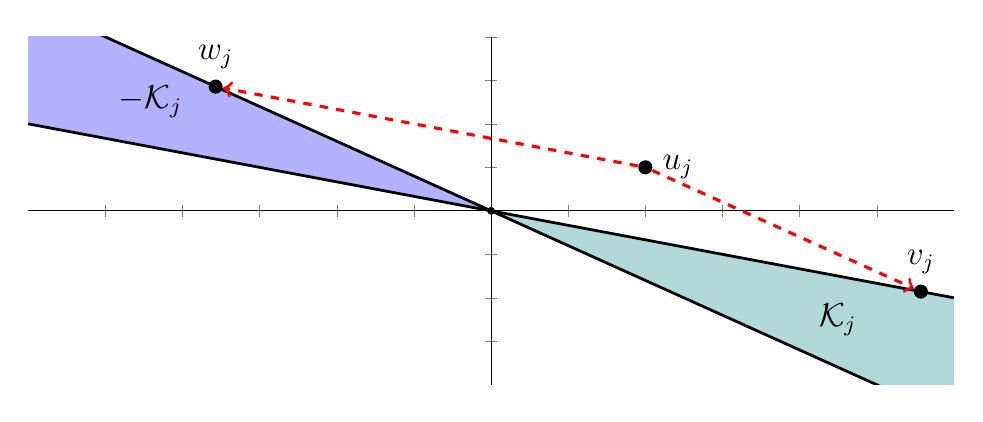
\begin{tikzpicture}[scale=1,
		declare function={
				cone_u(\x)= -\x/3;
				cone_l(\x)= -4*\x/5;
			}
	]
	\begin{axis}[width=1.1\linewidth, height=6cm,
			axis lines=center, yticklabels={,,}, xticklabels={,,},
			ymin=-4, ymax=4, ytick={-5,...,5}, ylabel=$$, x axis line style={-},
				xmin=-6, xmax=6, xtick={-5,...,5}, xlabel=$$, y axis line style={-},
		]
		\addplot[name path=cone_u, domain=-6:6, samples=100, line width=1pt]{cone_u(x)};
		\addplot[name path=cone_l, domain=-6:6, samples=200, line width=1pt]{cone_l(x)};

		% add color fill to both cones.
		\addplot fill between[
				of = cone_u and cone_l,
				split, % calculate segments
				every even segment/.style = {fill=blue, fill opacity=0.3},
				every odd segment/.style  = {fill=teal, fill opacity=0.3}
			];

		%% point labels
		% origin point
		\node[circle, fill, inner sep=1pt] at (axis cs:0,0) {};

		\node[label={0:$u_j$}, circle, fill, inner sep=1.8pt] (u) at (axis cs:2,1) {};
		\node[label={90:$v_j$}, circle, fill, inner sep=1.8pt] (v) at (axis cs:25/7+2, -25/21 - 2/3) {};
		\node[label={90:$w_j$}, circle, fill, inner sep=1.8pt] (w) at (axis cs:-25/7, 20/7) {};

		% labels
		\node[label={0:$\calK_j$}] at (axis cs:4,-2.5) {};
		\node[label={180:$-\calK_j$}] at (axis cs:-3.75,2.5) {};

		% lines
		\draw [->, dashed, draw=red, line width = 0.4mm] (u) edge (w);
		\draw [->, dashed, draw=red, line width = 0.4mm] (u) edge (v);
	\end{axis}

\end{tikzpicture}%

%        \else
%            \Huge cone decomp figure
%        \fi
%    \end{figure}

%\end{frame}
%\begin{frame}{Cone Decomposition: Basic Result}

%    \begin{beamercolorbox}[wd=\textwidth,sep=1em]{result}
%        \textbf{Proposition 3.1} (informal): If \( X \) is full row-rank,
%        then \( \text{aff}(\calK_j) = \R^d \) and
%        \( \calK_j - \calK_j = \R^d \).
%    \end{beamercolorbox}

%    \vspace{1em}

%    \pause
%    \begin{itemize}
%        \item Unfortunately, there is \bad{no extension} to full-rank \( X \).
%    \end{itemize}

%\end{frame}

%\begin{frame}{Cone Decompositions: Not All Cones are Equal}

%    \textbf{Alternative Idea}: show we don't need ``singular'' cones \( \calK_j \),
%    \[
%        \calK_j - \calK_j \subsetneq \R^d.
%    \]

%    \vspace{1em}
%    \pause

%    \begin{beamercolorbox}[wd=\textwidth,sep=1em]{result}
%        \textbf{Proposition 3.2} (informal): Suppose \( \calK_j - \calK_j \subset \R^d \).
%        Then, there exists \( \calK_i \) for which \( \calK_i - \calK_i = \R^d \)
%        and \( \calK_j \subset \calK_i \).
%    \end{beamercolorbox}

%    \pause
%    \vspace{1em}

%    \textbf{Interpretation}: if optimal \( u^*_j \neq 0 \), then set
%    \[
%        u_i' = u_j^* + u_i^*.
%    \]
%    It is possible to show this causes no problems.

%\end{frame}

%\begin{frame}{Cone Decomposition: Main Result}
%    \begin{itemize}
%        \item The proof is works by iteratively constructing a cone \( \calK_i \).
%              \vspace{0.2em}
%              \begin{itemize}
%                  \item Build \( \calK_i \) by flipping entries of \( D_j \).
%                        \vspace{0.2em}
%                  \item Equivalent to turning on/off activations.
%              \end{itemize}
%              \vspace{0.4em}

%        \item Leads to our main approximation result.
%    \end{itemize}

%    \pause
%    \horizontalrule

%    \begin{beamercolorbox}[wd=\textwidth,sep=1em]{result}
%        \textbf{Theorem 3.7} (informal):
%        Let \( \lambda \geq 0 \) and let \( p^* \) be the optimal value of the ReLU problem.
%        There exists a C-GReLU problem with minimizer \( u^* \) and optimal value \( d^* \) satisfying,
%        \[
%            d^* \leq p^* \leq d^* + \bad{2 \lambda \kappa(\tilde X_{\calJ}) \sum_{D_i \in \tilde \calD} \norm{u_i^*}_2}.
%        \]
%    \end{beamercolorbox}

%\end{frame}

%\begin{frame}{Cone Decompositions: Big Picture}
%    \begin{figure}[]
%        \centering
%        \ifdefined\showtikz
%            %! TEX root = ../../main.tex

%% illustration of relations between hypothesis classes. 

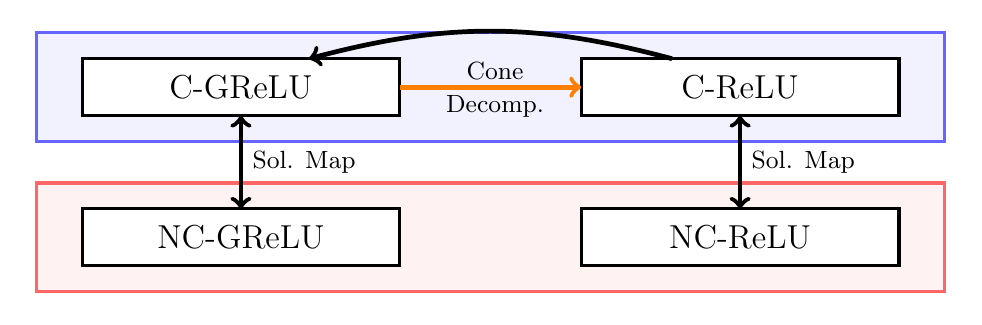
\begin{tikzpicture}[scale=1,
	]
	\begin{axis}[width=1.1\linewidth, height=5cm,
			axis lines=none,  % don't print axis lines
			yticklabels={,,}, xticklabels={,,},
			ymin=-0.2, ymax=10.2, x axis line style={-},
			xmin=-0.2, xmax=20.2, y axis line style={-},
		]

		\filldraw[color=blue!60, fill=blue!5, line width=0.4mm](axis cs:0,5.8) rectangle (axis cs:20, 10);
		\filldraw[color=red!60, fill=red!5, line width=0.4mm](axis cs:0,0) rectangle (axis cs:20, 4.2);

		% non-convex models
		\filldraw[line width=0.4mm, fill=white](axis cs:1,1) rectangle (axis cs:8, 3.2) node[pos=.5] {NC-GReLU};
		\filldraw[line width=0.4mm, fill=white](axis cs:12,1) rectangle (axis cs:19, 3.2) node[pos=.5] {NC-ReLU};

		% convex models
		\filldraw[line width=0.4mm, fill=white](axis cs:1,6.8) rectangle (axis cs:8, 9) node[pos=.5] {C-GReLU};
		\filldraw[line width=0.4mm, fill=white](axis cs:12,6.8) rectangle (axis cs:19, 9) node[pos=.5] {C-ReLU};

		\draw [<->, solid, draw=black, line width = 0.6mm] (axis cs:4.5,3.2) -- (axis cs:4.5,6.8) node[right, pos=0.5] {\small Sol. Map};

		\draw [<->, solid, draw=black, line width = 0.6mm] (axis cs:15.5,3.2) -- (axis cs:15.5,6.8)  node[right, pos=0.5] {\small Sol. Map};

        \draw [<-, solid, draw=black, line width = 0.6mm] (axis cs:6,9) to [bend left=15] (axis cs:14, 9);

		\draw [->, solid, draw=orange, line width = 0.6mm] (axis cs:8,7.9) -- (axis cs:12,7.9);
		\node[align=center] at (axis cs:10.1, 7.8) {\small Cone\\ \small Decomp.};
	\end{axis}

\end{tikzpicture}%

%        \else
%            \Huge Relations Figure
%        \fi
%    \end{figure}
%    \pause

%    \textbf{Takeaways}:

%    \vspace{0.5em}
%    \begin{itemize}
%        \item Gated ReLU and ReLU model classes are the same.
%        \item We can convert between them at will.
%    \end{itemize}
%\end{frame}

%\setbeamercolor{background canvas}{bg=LightCyan}

%\begin{frame}{}
%    \begin{center}
%        \huge IV. Solution Sets
%    \end{center}
%\end{frame}
%\setbeamercolor{background canvas}{bg=white}

%\begin{frame}{Model Problem: Constrained Group Lasso}

%    {
%        \large
%        \textbf{General Approach}:
%        \begin{enumerate}
%            \large
%            \item \pause
%                  Characterize solutions to the \good{convex reformulation}
%                  using strong duality and KKT conditions.
%                  \vspace{1ex}
%                  \pause
%            \item Extend results to \bad{non-convex} ReLU networks
%                  using the solution mapping.
%                  \vspace{1ex}
%                  \pause
%            \item Leverage explicit characterization of the optimal
%                  set for \good{new insights and algorithms}.
%        \end{enumerate}
%    }


%\end{frame}

%\begin{frame}{C-ReLU Optimal Set}

%    {\raggedright
%        1. Characterize solutions to the \good{convex reformulation}
%        using strong duality and KKT conditions.
%        \vspace{3ex}
%        \pause
%    }

%    \textbf{C-ReLU Solution Set}:
%    \[
%        \begin{aligned}
%            \solfn(\lambda) & =
%            \argmin_{v_i, w_i \in \calK_i} \, \bigg\{
%            \half \bigg\|\sum_{D_i \in \tilde \calD} D_i X (v_i - w_i), y\bigg\|_2^2                    \\
%                            & \quad \quad + \lambda\sum_{D_i \in \tilde \calD}\norm{v_i}_2+\norm{w_i}_2
%            \bigg\}.
%        \end{aligned}
%    \]

%    \pause
%    \horizontalrule

%    \begin{itemize}
%        \item Introduce dual variables \( \rho \) and analyze the KKT conditions.
%              \pause
%        \item Define
%              \(
%              \theta =
%              \begin{bmatrix}
%                  v_i \\
%                  -w_i
%              \end{bmatrix}.
%              \)

%        \item Index \( D_i's \) from \( 1 \) to \( 2p \).
%    \end{itemize}

%\end{frame}


%\begin{frame}{C-ReLU: the Optimal Set}
%    \vspace{-2ex}
%    \begin{itemize}
%        \item
%              \textbf{Optimal Fit: }       \( \hat y = \sum_{i=1}^{2p} D_i X \theta_i  \).
%              \pause
%              \vspace{1ex}

%        \item
%              \textbf{Block Correlation: } \( q_i = X^\top D_i (\hat y - y) - (2D_i - I)^\top \ri \).
%              \pause
%              \vspace{1ex}

%        \item
%              \textbf{Support Set: }      \( \calS_\lambda
%              = \cbr{\bi \in [2p] : \exists \theta \in \solfn(\lambda), \
%                  \theta_i \neq 0} \).
%    \end{itemize}

%    \vspace{-2ex}
%    \pause
%    \horizontalrule
%    \vspace{-1ex}

%    \begin{proposition}[Informal]
%        Fix \( \lambda > 0 \).
%        The optimal set of the C-ReLU problem is
%        given by
%        \begin{equation*}
%            \begin{aligned}
%                \solfn(\lambda) =
%                \big\{ & \theta  :
%                \forall \, \bi  \in  \calS_\lambda,
%                \theta_i =  \alpha_\bi q_i, \alpha_\bi \geq 0, \,             \\
%                       & \quad \forall \, j \in [2p] \setminus \calS_\lambda,
%                \theta_{j} = 0, \, \sum_{i=1}^{2p} D_i X \theta_i = \hat y
%                \big\}
%            \end{aligned}
%        \end{equation*}
%    \end{proposition}

%\end{frame}

%\begin{frame}{C-ReLU: Mapping back to Non-Convex Networks}

%    {\raggedright
%        2. Extend results to \bad{non-convex} ReLU networks
%        using the solution mapping.
%        \vspace{3ex}
%        \pause
%    }


%    \begin{corollary}[Informal]
%        Suppose \( m \geq m^* \).
%        Then the optimal set for the ReLU problem is
%        \vspace{-1ex}
%        \begin{equation*}
%            \begin{aligned}
%                \hspace{-0.5em} \calO_\lambda  = \,
%                \big\{
%                 & (W_1,  w_2) :
%                \, f_{W_1, w_2}(X)  =  \hat y,                       \\
%                 & \forall \, \bi  \in  \calS_\lambda,
%                W_{1i} = (\sfrac{\alpha_{i}}{\lambda})^{\sfrac{1}{2}} q_i,
%                w_{2i} = (\alpha_i \lambda)^{\sfrac{1}{2}},
%                \alpha_i \geq 0                                      \\
%                 & \forall \, \bi  \in [2p] \setminus \calS_\lambda,
%                W_{1i} = 0, \, w_{2i} = 0
%                \big\}.
%            \end{aligned}
%        \end{equation*}
%    \end{corollary}

%    \pause

%    We've derived the optimal set of the ReLU training problem!

%\end{frame}

%\begin{frame}{C-ReLU: Appearance of Solution Sets}
%    \begin{figure}[]
%        \centering
%        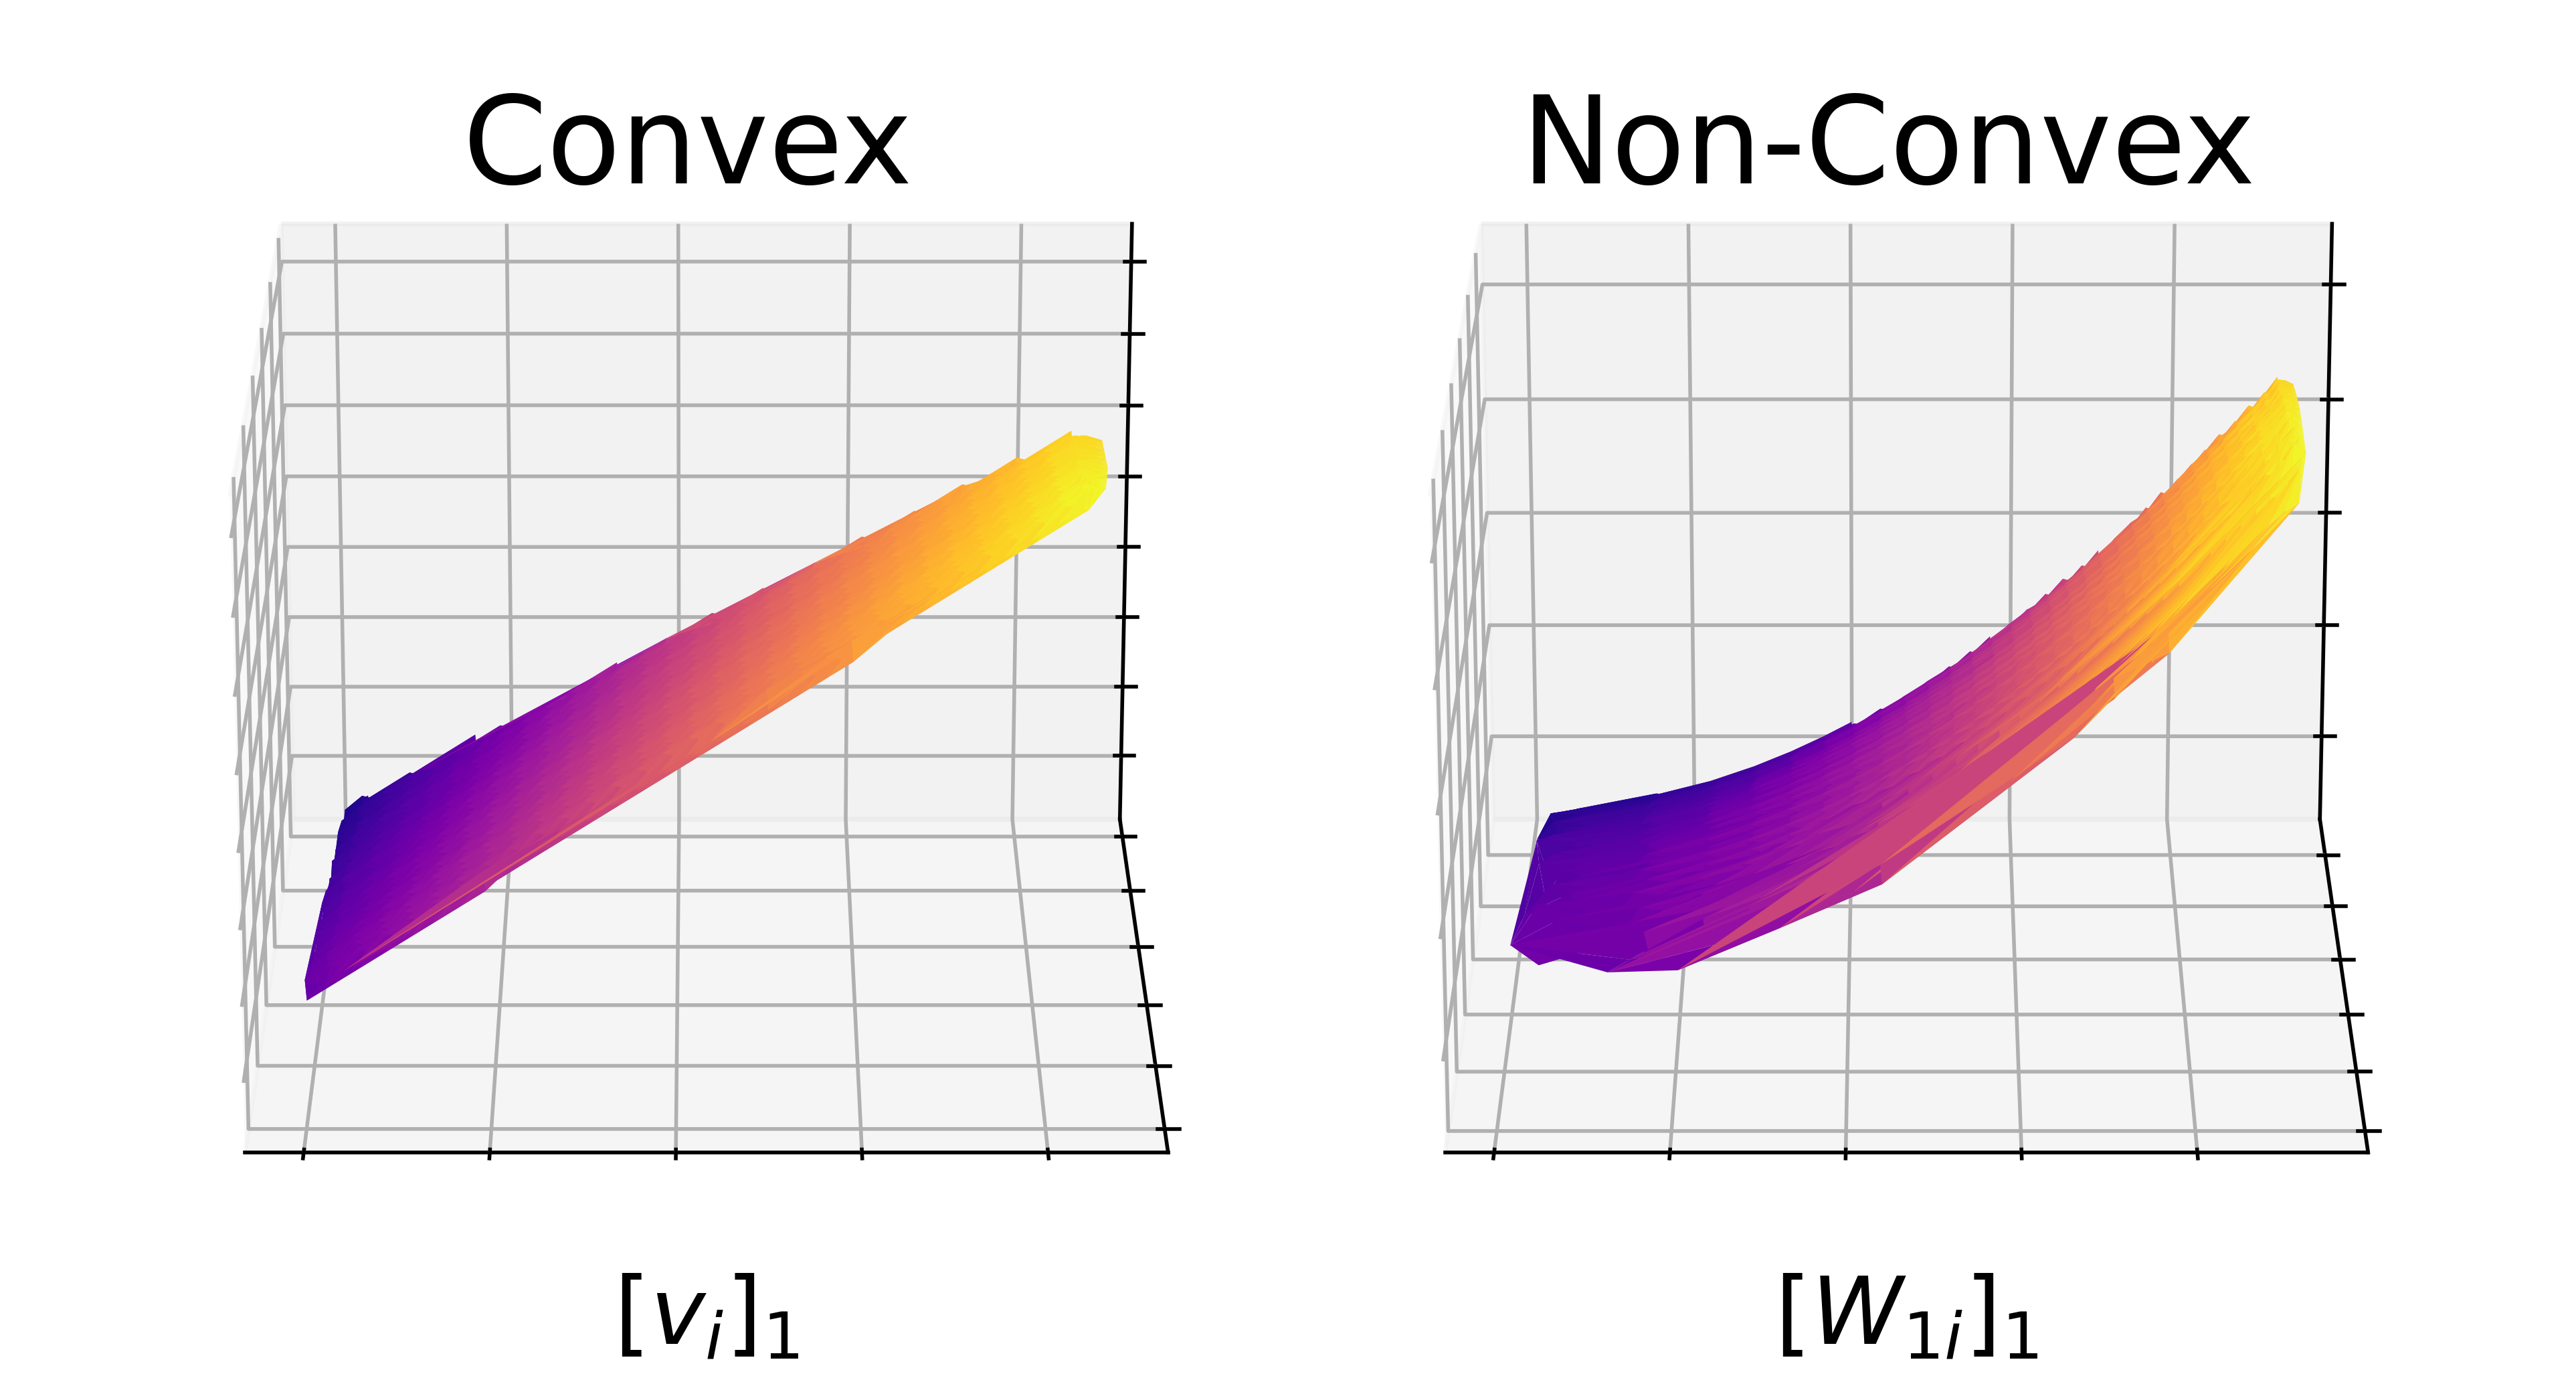
\includegraphics[width=0.96\textwidth]{assets/solution_sets_vis_270.png}
%    \end{figure}

%    \begin{itemize}
%        \item Non-convex parameterization maps polytope into curved
%              manifold.
%    \end{itemize}


%\end{frame}


%\begin{frame}{Optimal Pruning: Extreme Points}

%    {\raggedright
%        3. Leverage explicit characterization of the optimal
%        set for \good{new insights and algorithms}.
%        \vspace{3ex}
%        \pause
%    }

%    C-ReLU Optimal Set in \( \alpha \) space:
%    \begin{equation}
%        \begin{aligned}
%            \solfn(\lambda) & =
%            Q_{\calS_\lambda} \big\{ \alpha  : \sum_{i \in \calS_\lambda} (D_i X q_i) \alpha_i = \hat y,
%            \alpha_i \geq 0
%            \big\}                                                       \\
%                            & = Q_{\calS_\lambda} \calP_{\calS_\lambda}.
%        \end{aligned}
%    \end{equation}

%    \pause
%    \horizontalrule

%    \( \calP_{\calS_\lambda} \) is a polytope.
%    \pause
%    \begin{itemize}
%        \item \( \bar \alpha \in \calP_{\calS_\lambda} \) is a vertex
%              iff \( \cbr{D_i X q_i}_{\bar \alpha_i \neq 0} \) are linearly independent.
%              \pause
%        \item Are these vertices special somehow?
%    \end{itemize}

%\end{frame}

%\begin{frame}{Optimal Pruning: Algorithm}
%    \textbf{Definition}: A optimal C-ReLU model \( \theta \) is minimal
%    if there does
%    not exist another optimal model \( \theta' \) with strictly smaller support.

%    \vspace{3ex}
%    \pause

%    \begin{beamercolorbox}[wd=\textwidth,sep=1em]{result}
%        \textbf{Proposition 3.2} (informal):
%        For \( \lambda > 0 \), \( \theta \in \solfn(\lambda) \) is \good{minimal}
%        iff
%        the vectors \( \cbr{D_i X q_i}_{\alpha_i \neq 0} \)
%        are linearly independent.
%    \end{beamercolorbox}

%    \vspace{3ex}
%    \pause

%    \textbf{We prove}:
%    \begin{itemize}
%        \item Vertices of \( \solfn(\lambda) \) are minimal models.
%              \pause
%        \item All minimal models have the \good{same number} of active neurons.
%              \pause
%        \item There are at most \( n \) neurons in a minimal model.
%              \pause
%        \item Pruning from any optimal model will give a minimal model.
%    \end{itemize}

%\end{frame}

%\begin{frame}{Optimal Pruning: Pseudo-code}
%    \begin{algorithm}[H]
%        \caption{Pruning solutions}
%        \begin{algorithmic}
%            \STATE {\bfseries Input:} data matrix \( X \), solution \( \theta \).
%            \STATE \( k \gets 0 \).
%            \STATE \( \theta^k \gets \theta \).
%            \WHILE {\( \exists \beta \neq 0 \) s.t. \( \sum_{\bi \in \act(\theta^k)} \beta_\bi D_i X \theta_i^k = 0 \)}
%            \STATE \( \bi^k \gets \argmax_{\bi} \cbr{|\beta_\bi| : \bi \in \act(\theta^k)}  \)
%            \STATE \( t^k \gets 1/|\beta_{\bi^k}| \)
%            \STATE \( \theta^{k+1} \gets \theta^k (1 - t^k \beta_\bi) \)
%            \STATE \( k \gets k + 1 \)
%            \ENDWHILE
%            \STATE {\bfseries Output:} final weights \( \theta^k \)
%        \end{algorithmic}
%    \end{algorithm}

%    \pause

%    Let \( r = \text{rank}(X) \). Complexity to compute a minimal model:

%    \[ O\rbr{d^3 r^3 (\frac{n}{r})^{3r} + \good{(n^3 + nd) r (\frac{n}{r})^r}}. \]

%\end{frame}

%\setbeamercolor{background canvas}{bg=LightCyan}

%\begin{frame}{}
%    \begin{center}
%        \huge V. Experimental Results
%    \end{center}
%\end{frame}
%\setbeamercolor{background canvas}{bg=white}

%\begin{frame}{Algorithms: Solving the Convex Programs}
%    We develop two algorithms for solving the convex reformulations:

%    \vspace{1em}

%    \begin{itemize}
%        \item \textbf{R-FISTA}: a restarted FISTA variant for Gated ReLU.
%              \vspace{0.5em}
%        \item \textbf{AL}: an augmented Lagrangian method for the (constrained) ReLU Problem.
%    \end{itemize}

%    \pause
%    \horizontalrule

%    And we can use all the convex tricks!
%    \vspace{1em}
%    \begin{itemize}
%        \item \textbf{Fast}: \( O(1/T^2) \) convergence rate.
%              \vspace{0.5em}

%        \item \textbf{Tuning-free}: line-search, restarts, data normalization, \ldots
%              \vspace{0.5em}

%        \item \textbf{Certificates}: termination based on min-norm subgradient.
%    \end{itemize}

%\end{frame}

%\begin{frame}{Algorithms: Optimization Performance}
%    \begin{figure}[t]
%        \centering
%        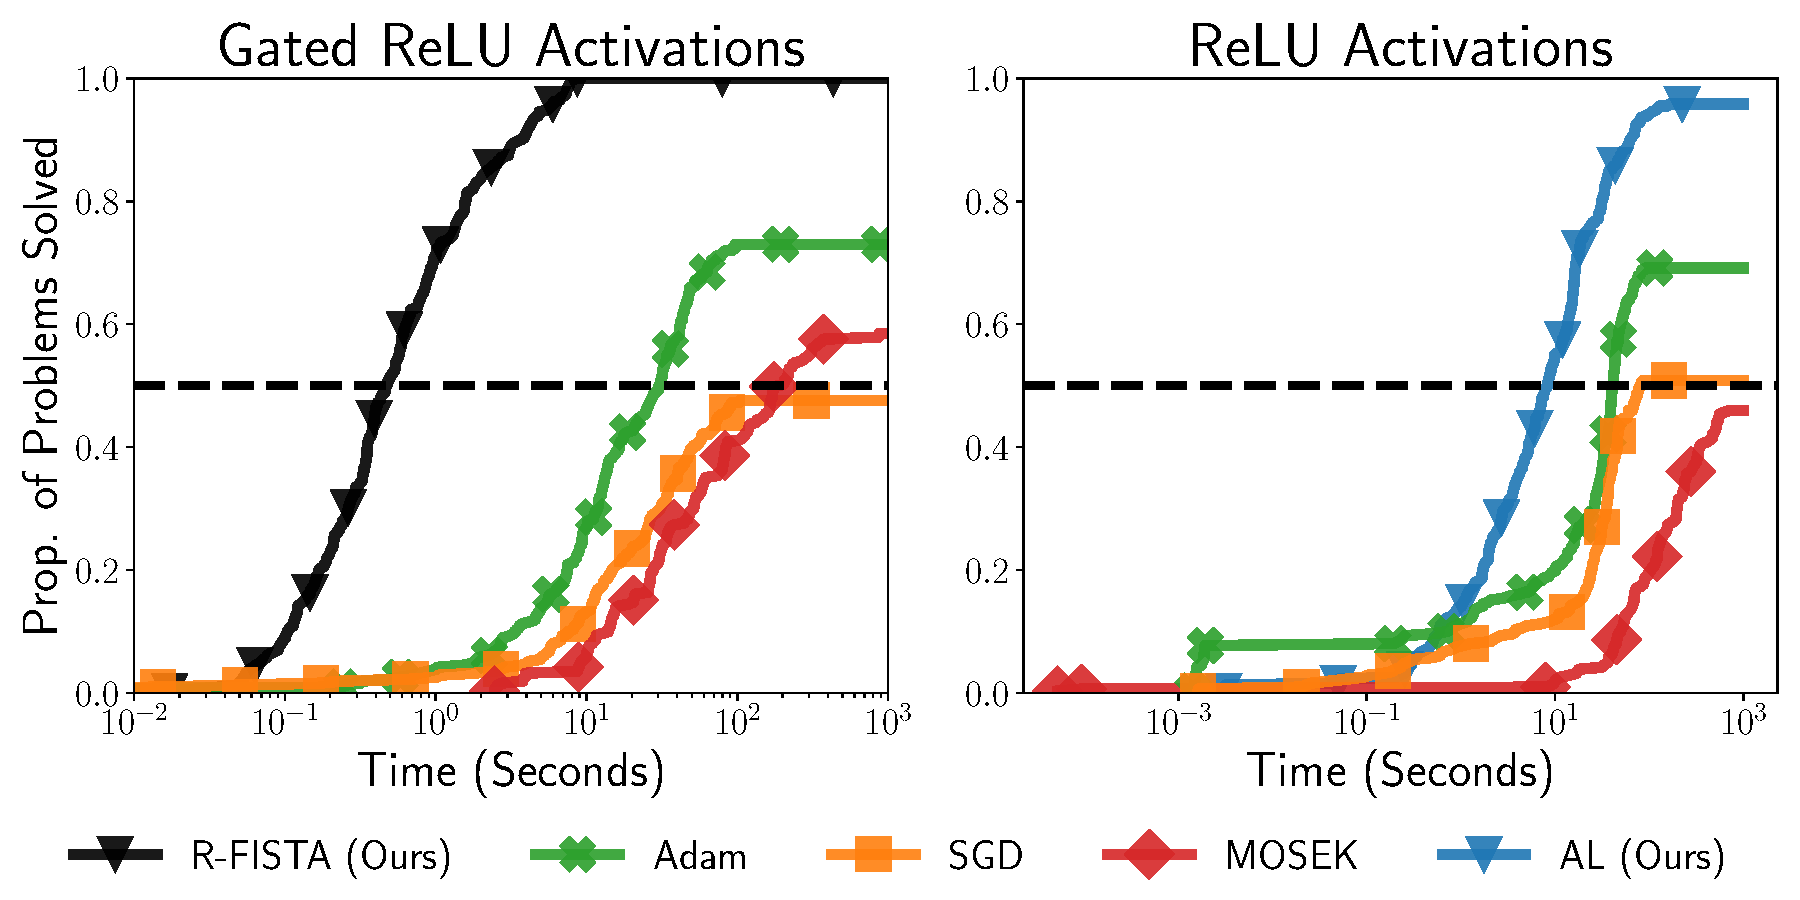
\includegraphics[width=1\linewidth]{assets/pp_main.pdf}
%    \end{figure}
%    \begin{itemize}
%        \item Generated by 438 training problems taken from UCI repo.
%        \item R-FISTA/AL solve more, faster, than SGD and Adam.
%    \end{itemize}
%\end{frame}

%\begin{frame}{Algorithms: Exploring the Optimal Set}

%    \begin{figure}[t]
%        \centering
%        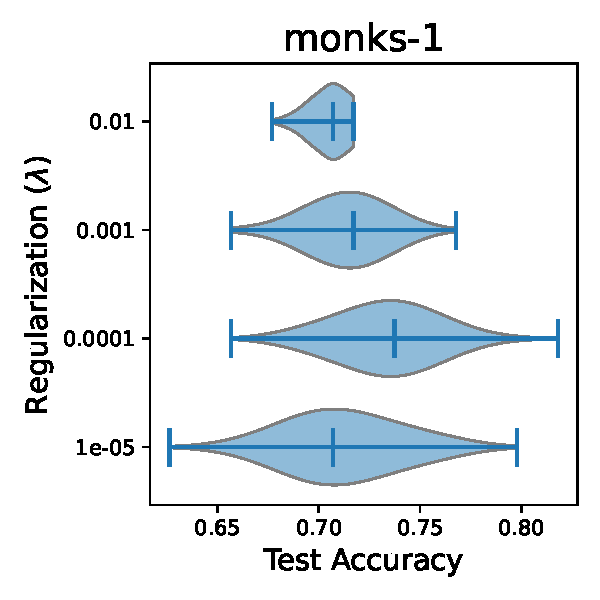
\includegraphics[width=0.48\linewidth]{assets/dist_paper_monks-1.pdf}
%        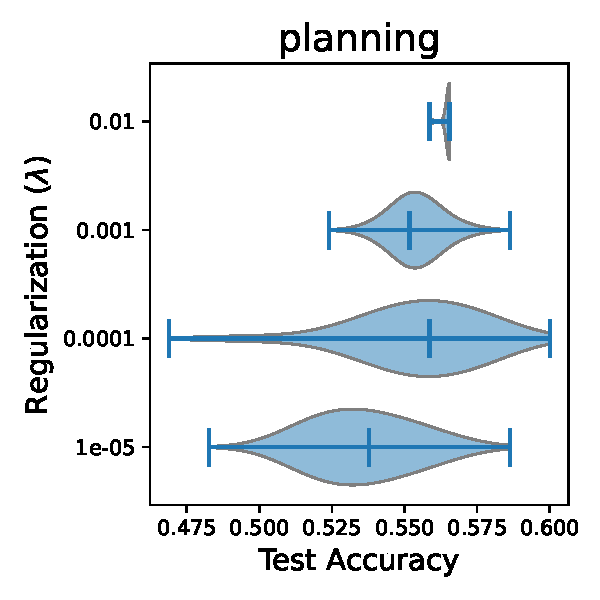
\includegraphics[width=0.48\linewidth]{assets/dist_paper_planning.pdf}
%    \end{figure}
%    \begin{itemize}
%        \item Take 10,000 samples from the set of optimal neural networks.
%        \item All samples have (i) \textbf{same training accuracy},
%              (ii)~\textbf{same model norm}, but generalize very differently.
%    \end{itemize}
%\end{frame}

%\begin{frame}{Algorithms: (Sub)-Optimal Pruning}
%    \begin{figure}[t]
%        \centering
%        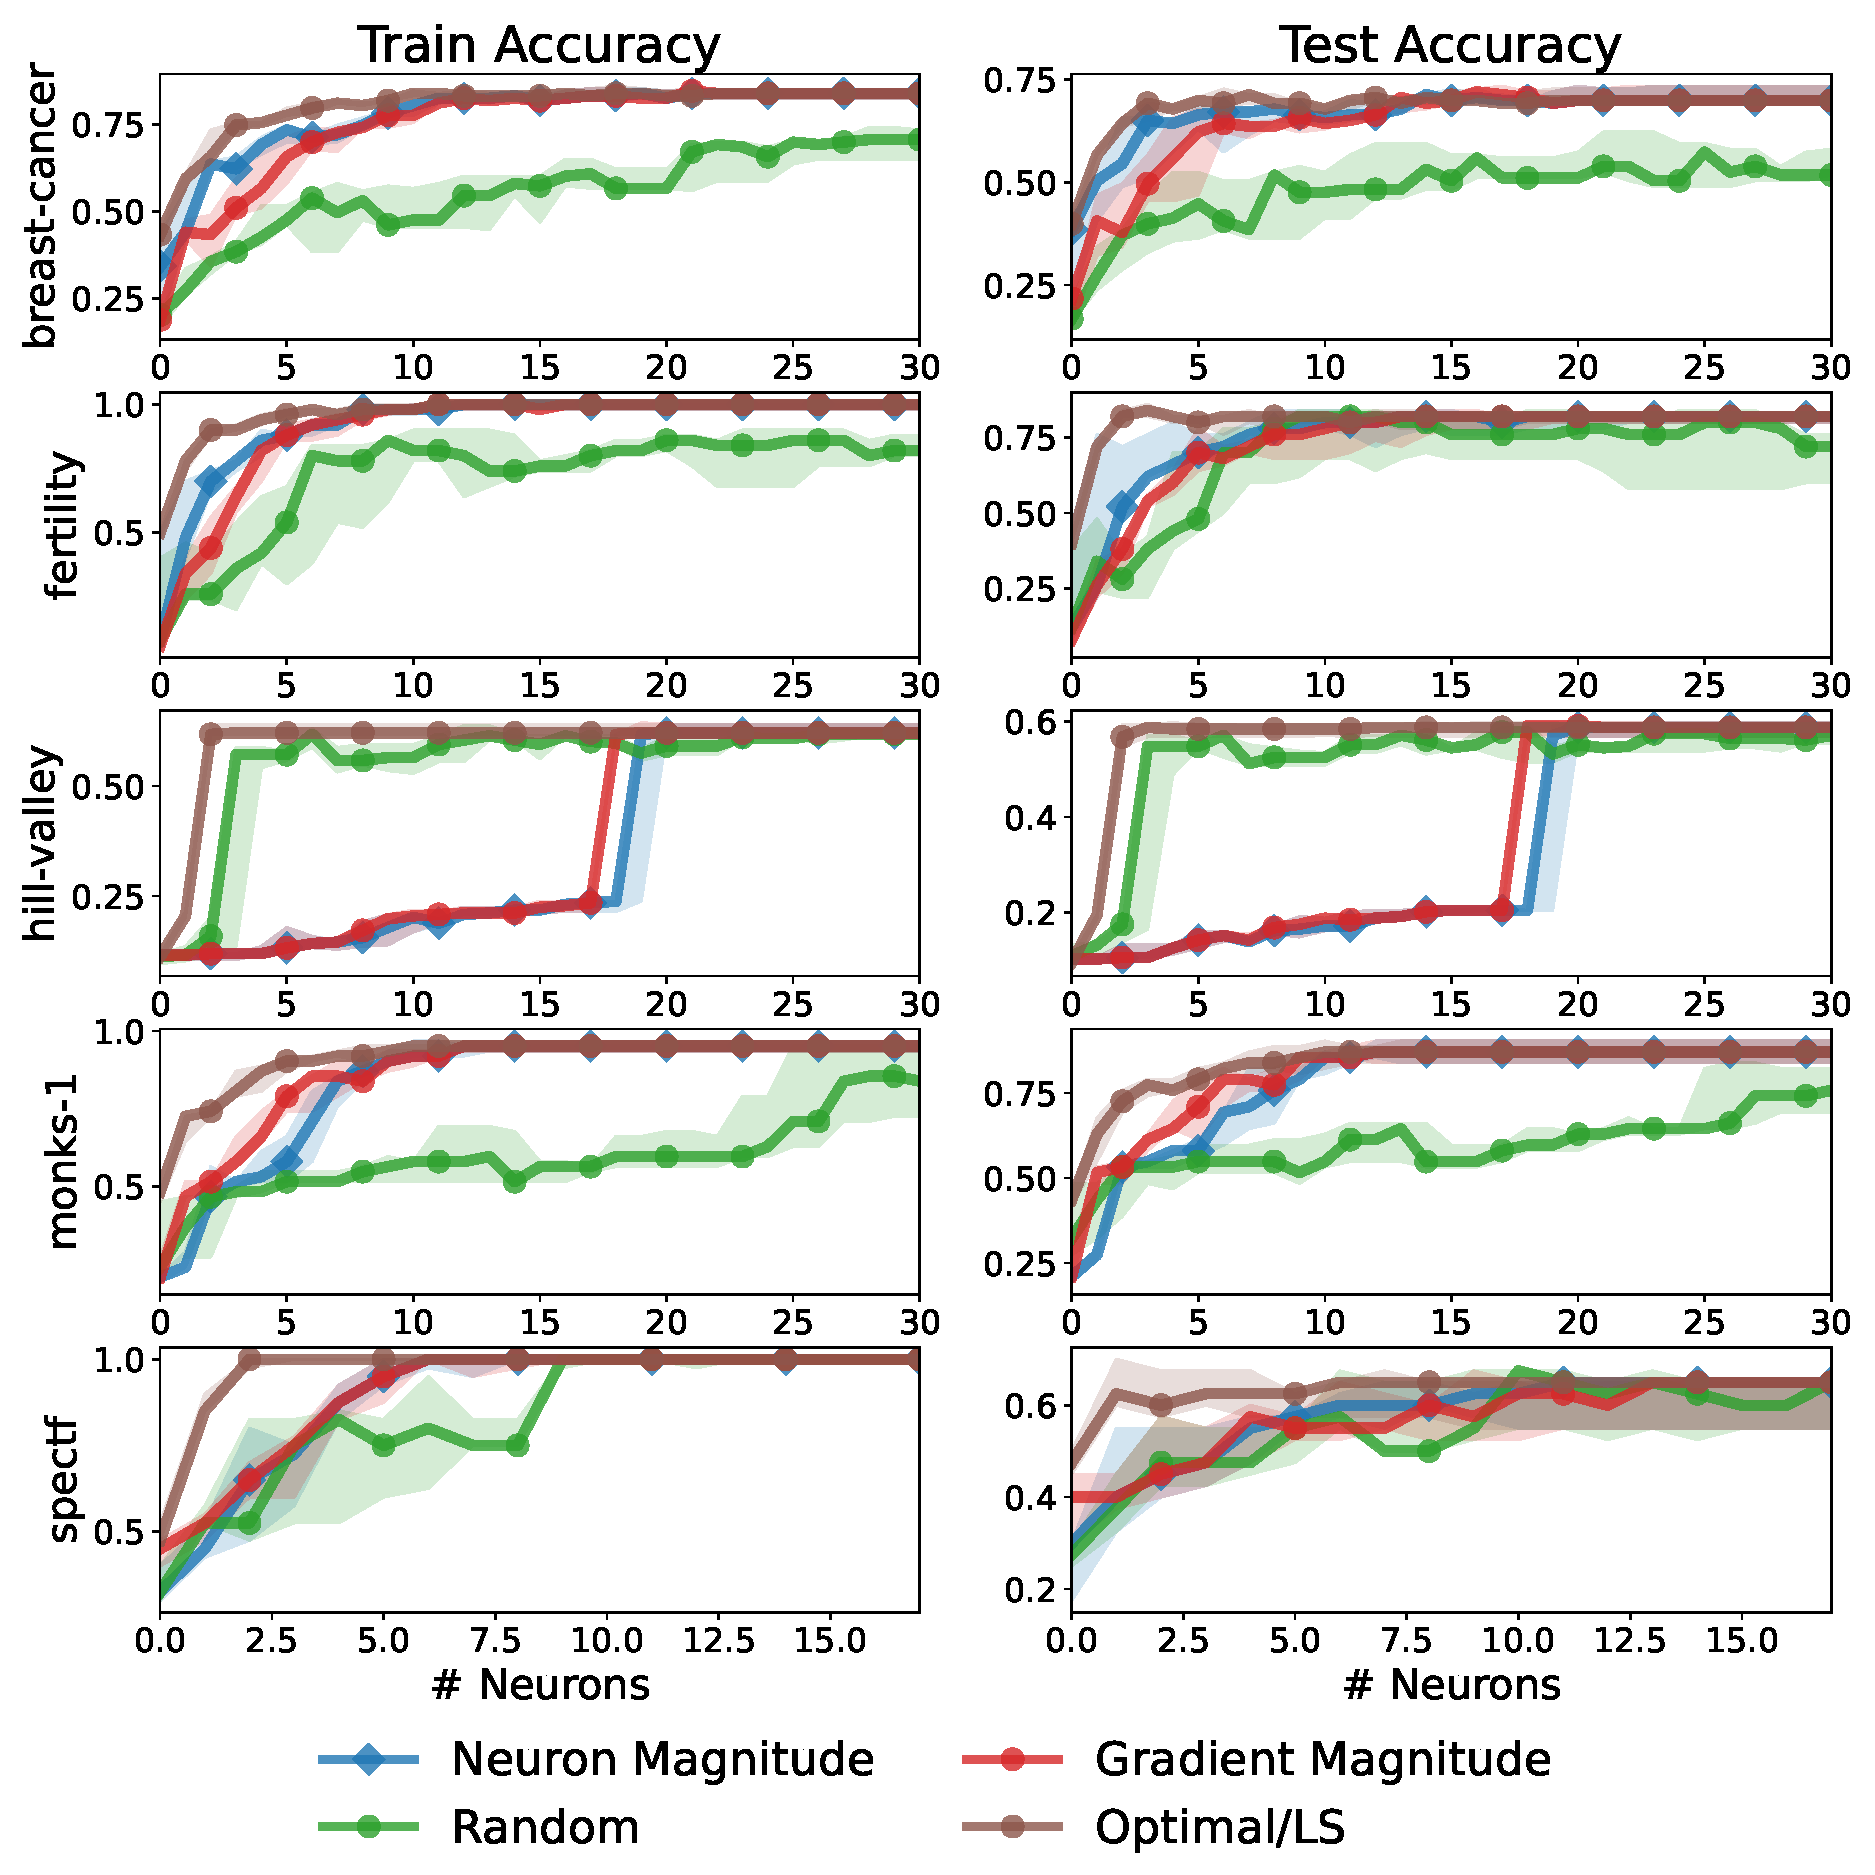
\includegraphics[width=0.75\textwidth]{assets/uci_pruning_full_paper.pdf}
%    \end{figure}
%\end{frame}

%\begin{frame}{Algorithms: (Sub)-Optimal Pruning}
%    \begin{figure}[t]
%        \centering
%        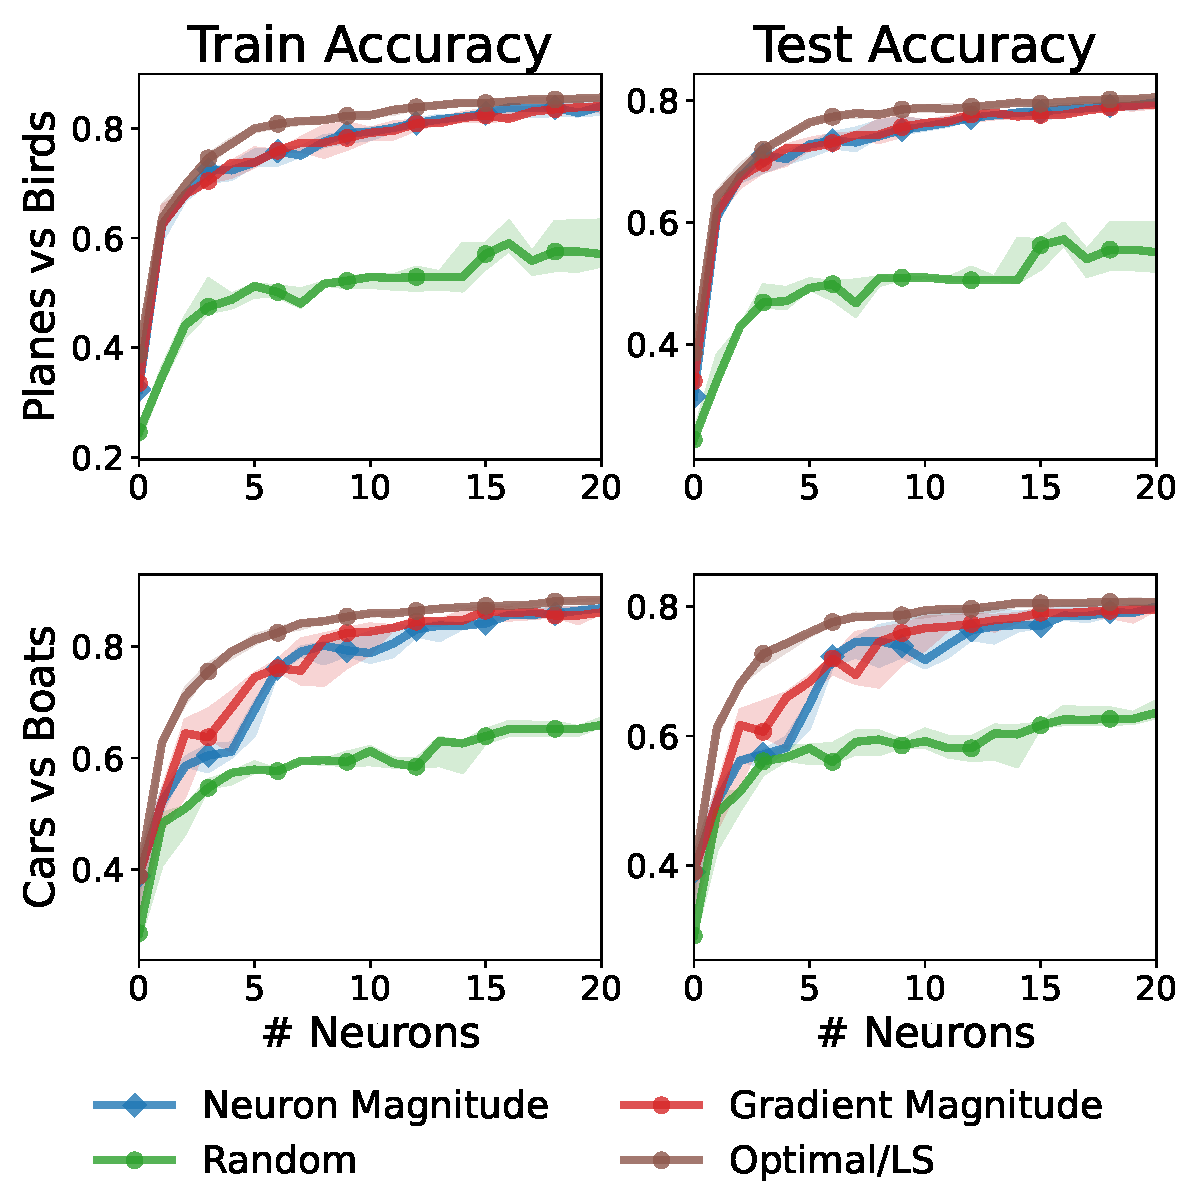
\includegraphics[width=0.75\textwidth]{assets/prune_cifar.pdf}
%    \end{figure}
%\end{frame}

%\setbeamercolor{background canvas}{bg=LightCyan}

%\begin{frame}{}
%    \begin{center}
%        \huge Pause.
%    \end{center}
%\end{frame}
%\setbeamercolor{background canvas}{bg=white}

%\begin{frame}{Recap}
%    \begin{center}
%        \huge   Our Contributions.
%    \end{center}

%    \vspace{2em}
%    \pause
%    { \large
%        \begin{itemize}
%            \item We approximate the ReLU training problem by \textbf{unconstrained}
%                  convex optimization of a Gated ReLU network.\pause
%                  \vspace{0.5em}

%            \item We leverage convex reformulations to \textbf{analyze} the set
%                  of optimal ReLU networks.
%                  \pause
%                  \vspace{0.5em}

%            \item We propose and \textbf{exhaustively evaluate} algorithms for solving
%                  convex reformulations.
%        \end{itemize}
%    }

%\end{frame}


%%% main content ends %%

%%% end slide
%\setbeamercolor{background canvas}{bg=LightCyan}

%\begin{frame}{}
%    \begin{center}
%        \huge Try our Code!
%    \end{center}

%    \begin{figure}[]
%        \centering
%        
\includegraphics[width=0.6\textwidth]{assets/github.png}
%    \end{figure}
%\end{frame}
%\setbeamercolor{background canvas}{bg=white}

%%% bibliography
%\begin{frame}[allowframebreaks]{References}
%    \printbibliography[]
%\end{frame}


%\begin{frame}{Bonus: Cone Decomposition Proof Sketch}

%    \begin{beamercolorbox}[wd=\textwidth,sep=1em]{result}
%        \textbf{Proposition 3.2} (informal): Suppose \( \calK_j - \calK_j \subset \R^d \).
%        Then, there exists \( \calK_i \) for which \( \calK_i - \calK_i = \R^d \)
%        and \( \calK_j \subset \calK_i \).
%    \end{beamercolorbox}

%    \pause
%    \vspace{1em}

%    \textbf{Recall}: \( \calK_j = \cbr{w : (2 D_j - I) X w \geq 0} \).
%    \pause

%    \begin{itemize}
%        \item This is a polyhedral cone which we rewrite as
%              \[
%                  \calK_j = \bigcap_{i=1}^n \cbr{w : [S_j]_{ii} \cdot \abr{x_i, w} \geq 0},
%              \]
%              where \( S_j = (2D_j - I) \).
%    \end{itemize}
%\end{frame}

%\begin{frame}{Bonus: Cone Decomposition Proof Sketch}

%    \begin{beamercolorbox}[wd=\textwidth,sep=1em]{result}
%        \textbf{Proposition 3.2} (informal): Suppose \( \calK_j - \calK_j \subset \R^d \).
%        Then, there exists \( \calK_i \) for which \( \calK_i - \calK_i = \R^d \)
%        and \( \calK_j \subset \calK_i \).
%    \end{beamercolorbox}

%    \vspace{2ex}

%    \textbf{Proof}: Works by iteratively constructing \( \calK_i \) s.t. \( \calK_j \subset \calK_i \).

%    \pause
%    \horizontalrule

%    We sketch a simpler statement:

%    \vspace{1em}

%    \begin{beamercolorbox}[wd=\textwidth,sep=1em]{relaxation}
%        \textbf{Proposition 3.2} (informal): Suppose \( \calK_j = \cbr{0} \).
%        Then, there exists \( \calK_i \) for which \( \calK_i - \calK_i = \R^d \)
%        and \( \calK_j \subset \calK_i \).
%    \end{beamercolorbox}


%\end{frame}


%\begin{frame}{Bonus: Cone Decomposition Proof Sketch}
%    \[
%        \calK_j' = \cbr{w : [S_j]_{11} \cdot \abr{x_1, w} \geq 0}
%    \]
%    \begin{figure}[]
%        \centering
%        \ifdefined\showtikz
%            %! TEX root = ../../main.tex

%% Illustration of cone decomposition. 

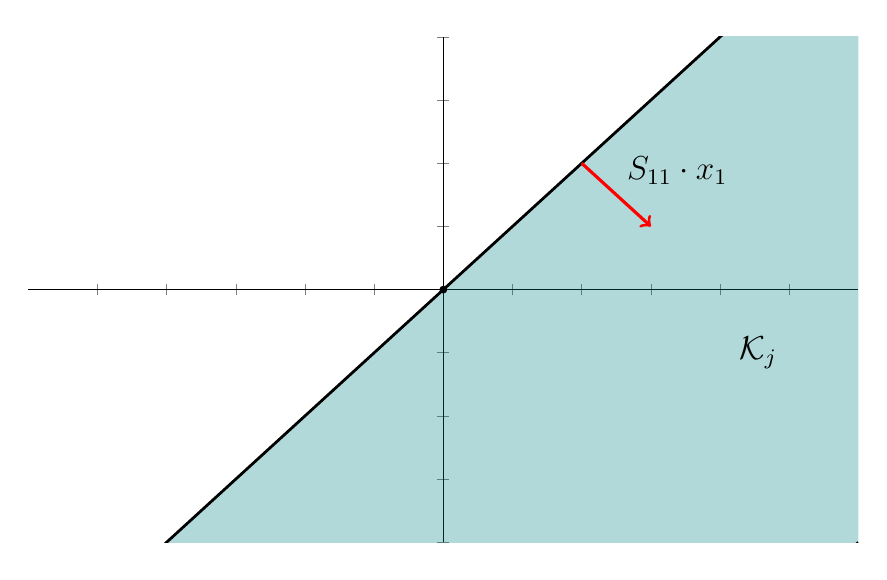
\begin{tikzpicture}[scale=1,
		declare function={
				cone_1(\x)= \x;
				cone_2(\x)= -\x;
				cone_3(\x)= -4*\x;
				bounds(\x)= \x - 10;
			}
	]
	\begin{axis}[width=\linewidth, height=8cm,
			axis lines=center, yticklabels={,,}, xticklabels={,,},
			ymin=-4, ymax=4, ytick={-5,...,5}, ylabel=$$, x axis line style={-},
				xmin=-6, xmax=6, xtick={-5,...,5}, xlabel=$$, y axis line style={-},
		]
		\addplot[name path=cone_1, domain=-6:6, samples=100, line width=1pt]{cone_1(x)};
		%\addplot[name path=cone_2, domain=-6:6, samples=200, line width=1pt]{cone_2(x)};
		%\addplot[name path=cone_3, domain=-6:6, samples=200, line width=1pt]{cone_3(x)};
		\addplot[name path=bounds, domain=-6:6, samples=100, line width=1pt]{bounds(x)};

		% add color fill to both cones.

		\addplot fill between[
				of = cone_1 and bounds,
				%split, % calculate segment
				every even segment/.style = {fill=teal, fill opacity=0.3},
			];

		%% point labels
		% origin point
		\node[circle, fill, inner sep=1pt] at (axis cs:0,0) {};

		% labels
		\node[label={0:$\calK_j$}] at (axis cs:4,-1) {};

		% lines
        \draw [->, draw=red, line width = 0.4mm] (axis cs:2,2) -- (axis cs:3,1) node[midway,above right] {$S_{11} \cdot x_1$};
		%\draw [->, draw=red, line width = 0.4mm] (axis cs:2,-2) -- (axis cs:3,-1) node[midway,below right] {$S_{22} \cdot x_2$};
		%\draw [->, draw=red, line width = 0.4mm] (axis cs:0.5,-2) -- (axis cs:-2.5,-2.75) node[pos=0.9,below right] {$S_{33} \cdot x_3$};
	\end{axis}

\end{tikzpicture}%

%        \else
%            \Huge Empty cone figure
%        \fi
%    \end{figure}
%\end{frame}

%\begin{frame}{Bonus: Cone Decompositions Proof Sketch}

%    \[
%        \calK_j'' = \calK_j' \cap \cbr{w : [S_j]_{22} \cdot \abr{x_2, w} \geq 0}
%    \]

%    \begin{figure}[]
%        \centering
%        \ifdefined\showtikz
%            %! TEX root = ../../main.tex

%% Illustration of cone decomposition. 

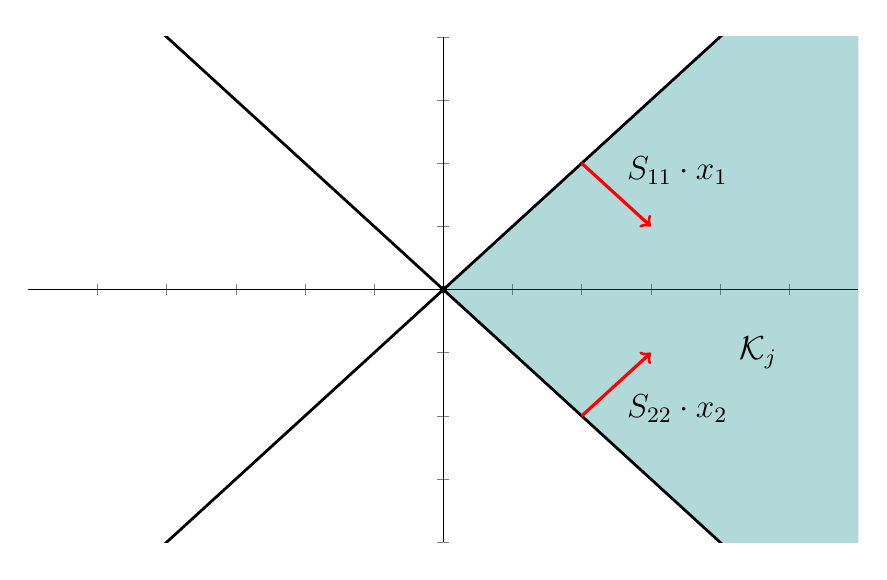
\begin{tikzpicture}[scale=1,
		declare function={
				cone_1(\x)= \x;
				cone_2(\x)= -\x;
				cone_3(\x)= -4*\x;
			}
	]
	\begin{axis}[width=\linewidth, height=8cm,
			axis lines=center, yticklabels={,,}, xticklabels={,,},
			ymin=-4, ymax=4, ytick={-5,...,5}, ylabel=$$, x axis line style={-},
				xmin=-6, xmax=6, xtick={-5,...,5}, xlabel=$$, y axis line style={-},
		]
		\addplot[name path=cone_1, domain=-6:6, samples=100, line width=1pt]{cone_1(x)};
		\addplot[name path=cone_2, domain=-6:6, samples=200, line width=1pt]{cone_2(x)};
		%\addplot[name path=cone_3, domain=-6:6, samples=200, line width=1pt]{cone_3(x)};

		% add color fill to both cones.
		\addplot fill between[
				of = cone_1 and cone_2,
				split, % calculate segments
				every even segment/.style = {fill=blue, fill opacity=0},
				every odd segment/.style  = {fill=teal, fill opacity=0.3}
			];

		%% point labels
		% origin point
		\node[circle, fill, inner sep=1pt] at (axis cs:0,0) {};

		% labels
		\node[label={0:$\calK_j$}] at (axis cs:4,-1) {};

		% lines
        \draw [->, draw=red, line width = 0.4mm] (axis cs:2,2) -- (axis cs:3,1) node[midway,above right] {$S_{11} \cdot x_1$};
		\draw [->, draw=red, line width = 0.4mm] (axis cs:2,-2) -- (axis cs:3,-1) node[midway,below right] {$S_{22} \cdot x_2$};
		%\draw [->, draw=red, line width = 0.4mm] (axis cs:0.5,-2) -- (axis cs:-2.5,-2.75) node[pos=0.9,below right] {$S_{33} \cdot x_3$};
	\end{axis}

\end{tikzpicture}%

%        \else
%            \Huge Empty cone figure
%        \fi
%    \end{figure}
%\end{frame}


%\begin{frame}{Bonus: Cone Decomposition Proof Sketch}

%    \[
%        \calK_j''' = \calK_j'' \cap \cbr{w : [S_j]_{33} \cdot \abr{x_3, w} \geq 0}
%    \]

%    \begin{figure}[]
%        \centering
%        \ifdefined\showtikz
%            %! TEX root = ../../main.tex

%% Illustration of cone decomposition. 

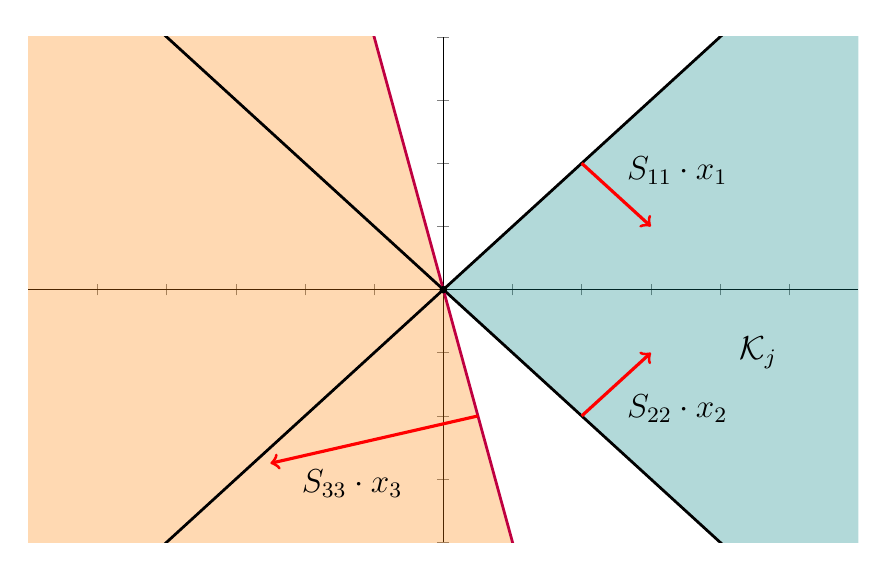
\begin{tikzpicture}[scale=1,
		declare function={
				cone_1(\x)= \x;
				cone_2(\x)= -\x;
				cone_3(\x)= -4*\x;
				bounds(\x)= -4*\x - 100;
			}
	]
	\begin{axis}[width=\linewidth, height=8cm,
			axis lines=center, yticklabels={,,}, xticklabels={,,},
			ymin=-4, ymax=4, ytick={-5,...,5}, ylabel=$$, x axis line style={-},
				xmin=-6, xmax=6, xtick={-5,...,5}, xlabel=$$, y axis line style={-},
		]
		\addplot[name path=cone_1, domain=-6:6, samples=100, line width=1pt]{cone_1(x)};
		\addplot[name path=cone_2, domain=-6:6, samples=200, line width=1pt]{cone_2(x)};
		\addplot[name path=cone_3, domain=-6:6, samples=200, line width=1pt, draw=purple]{cone_3(x)};
		\addplot[name path=bounds, domain=-6:6, samples=200, line width=1pt]{bounds(x)};

		% add color fill to both cones.
		\addplot fill between[
				of = cone_1 and cone_2,
				split, % calculate segments
				every even segment/.style = {fill=blue, fill opacity=0},
				every odd segment/.style  = {fill=teal, fill opacity=0.3}
			];

		\addplot fill between[
				of = cone_3 and bounds,
				every even segment/.style = {fill=orange, fill opacity=0.3},
			];

		%% point labels
		% origin point
		\node[circle, fill, inner sep=1pt] at (axis cs:0,0) {};

		% labels
		\node[label={0:$\calK_j$}] at (axis cs:4,-1) {};

		% lines
        \draw [->, draw=red, line width = 0.4mm] (axis cs:2,2) -- (axis cs:3,1) node[midway,above right] {$S_{11} \cdot x_1$};
		\draw [->, draw=red, line width = 0.4mm] (axis cs:2,-2) -- (axis cs:3,-1) node[midway,below right] {$S_{22} \cdot x_2$};
		\draw [->, draw=red, line width = 0.4mm] (axis cs:0.5,-2) -- (axis cs:-2.5,-2.75) node[pos=0.9,below right] {$S_{33} \cdot x_3$};
	\end{axis}

\end{tikzpicture}%

%        \else
%            \Huge empty cone figure
%        \fi
%    \end{figure}
%\end{frame}


%\begin{frame}{Bonus: Cone Decomposition Proof Sketch}

%    \[
%        \tilde \calK_j''' = \calK_j'' \cap \cbr{w : -[S_j]_{33} \cdot \abr{x_3, w} \geq 0}
%    \]

%    \begin{figure}[]
%        \centering
%        \ifdefined\showtikz
%            %! TEX root = ../../main.tex

%% Illustration of cone decomposition. 

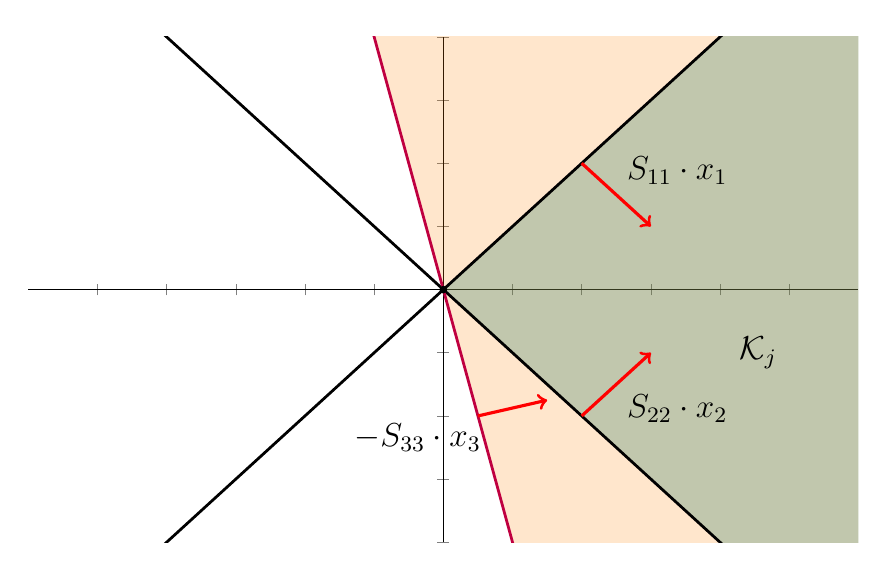
\begin{tikzpicture}[scale=1,
		declare function={
				cone_1(\x)= \x;
				cone_2(\x)= -\x;
				cone_3(\x)= -4*\x;
				bounds(\x)= -4*\x + 100;
			}
	]
	\begin{axis}[width=\linewidth, height=8cm,
			axis lines=center, yticklabels={,,}, xticklabels={,,},
			ymin=-4, ymax=4, ytick={-5,...,5}, ylabel=$$, x axis line style={-},
				xmin=-6, xmax=6, xtick={-5,...,5}, xlabel=$$, y axis line style={-},
		]
		\addplot[name path=cone_1, domain=-6:6, samples=100, line width=1pt]{cone_1(x)};
		\addplot[name path=cone_2, domain=-6:6, samples=200, line width=1pt]{cone_2(x)};
		\addplot[name path=cone_3, domain=-6:6, samples=200, line width=1pt, draw=purple]{cone_3(x)};
		\addplot[name path=bounds, domain=-6:6, samples=200, line width=1pt]{bounds(x)};

		% add color fill to both cones.
		\addplot fill between[
				of = cone_1 and cone_2,
				split, % calculate segments
				every even segment/.style = {fill=blue, fill opacity=0},
				every odd segment/.style  = {fill=teal, fill opacity=0.3}
			];

		\addplot fill between[
				of = cone_3 and bounds,
				every even segment/.style = {fill=orange, fill opacity=0.2},
			];

		%% point labels
		% origin point
		\node[circle, fill, inner sep=1pt] at (axis cs:0,0) {};

		% labels
		\node[label={0:$\calK_j$}] at (axis cs:4,-1) {};

		% lines
        \draw [->, draw=red, line width = 0.4mm] (axis cs:2,2) -- (axis cs:3,1) node[midway,above right] {$S_{11} \cdot x_1$};
		\draw [->, draw=red, line width = 0.4mm] (axis cs:2,-2) -- (axis cs:3,-1) node[midway,below right] {$S_{22} \cdot x_2$};
		\draw [->, draw=red, line width = 0.4mm] (axis cs:0.5,-2) -- (axis cs:1.5,-1.75) node[pos=0.2,below left] {$-S_{33} \cdot x_3$};
	\end{axis}

\end{tikzpicture}%

%        \else
%            \Huge Empty cone figure
%        \fi
%    \end{figure}
%\end{frame}

%\begin{frame}{Bonus: C-ReLU Optimality Conditions}

%    We form the Lagrangian for the convex reformulation:

%    \begin{equation*}
%        \begin{aligned}
%            \calL(v, w, \rho^{+}, \rho^{-})
%             & = \half \norm{\sum_{D_i \in \tilde \calD} D_i X (v_i - w_i) - y}_2^2
%            + \lambda\sum_{D_i \in \tilde \calD}\norm{v_i}_2 + \norm{w_i}_2                  \\
%             & \quad \quad - \sum_{D_i \tilde \calD} \sbr{\abr{\tilde{X_i}^\top \rho^{-}, w}
%                - \abr{\tilde{X_i}^\top \rho^{+}, v}},
%        \end{aligned}
%    \end{equation*}

%    where \( \tilde X_{i} = (2D_i - I) \).

%    \pause
%    \horizontalrule

%    The \good{KKT conditions} are necessary and sufficient for optimality:\pause

%    \vspace{1ex}
%    \begin{itemize}
%        \item Stationary Lagrangian:
%              \[
%                  \underbrace{X^\top D_i (\hat y - y) - \tilde{X_i}^\top \ri^{+}}_{q_i^+} \in \partial \lambda \norm{v_i}_2.
%              \]
%              \pause
%              \begin{itemize}
%                  \normalsize
%                  \item It turns out each \( q_i^+ \) is \textbf{unique} WLOG!
%              \end{itemize}
%    \end{itemize}

%\end{frame}

%\begin{frame}{Bonus: Characterizing the Optimal Set}

%    \textbf{Facts}: let \( (\theta, \rho) \) be primal dual optimal. \pause
%    \begin{itemize}
%        \item Model fit \( \hat y \) is \good{constant} over optimal set \( \solfn(\lambda) \). \pause
%        \item Implies correlation \( X^\top D_i (y - \hat y) \) is \good{constant} over \( \solfn(\lambda) \). \pause
%        \item We may assume \( \rho \) is \good{unique} (e.g. min-norm dual solution).
%    \end{itemize}

%    \pause
%    \horizontalrule

%    \textbf{Non-zero Blocks}:
%    \begin{itemize}
%        \item Suppose \( \theta_i \neq 0 \).
%              \pause
%        \item Then \( \nabla \norm{\theta_i}_2 = s_\bi = \lambda \theta_i / \norm{\theta_i}_2 \).
%              \pause
%        \item Rearranging stationarity implies \( \exists \alpha_\bi > 0 \):
%              \[
%                  \theta_i = \good{\alpha_\bi} \underbrace{\sbr{X^\top D_i (y - \hat y) - \tilde X_i \ri}}_{q_i}.
%              \]
%              \pause
%        \item Every solution is a non-negative multiple of these \( q_i \) vectors.
%    \end{itemize}

%\end{frame}

%\begin{frame}{Bonus: Explicit Optimal Set}
%    We gave a characterization of \( \solfn(\lambda) \) that depends on
%    \[
%        \calS_\lambda
%        = \cbr{\bi \in [2p] : \exists \theta \in \solfn(\lambda), \
%            \theta_i \neq 0}.
%    \]

%    Alternative expression involves additional linear constraints.

%    \pause
%    \horizontalrule

%    \begin{equation*}
%        \begin{aligned}
%            \solfn(\lambda) =
%            \big\{ & \theta  :
%            \forall \, \bi  \in  \equi,
%            \theta_i =  \alpha_\bi q_i, \alpha_\bi \geq 0, \,           \\
%                   & \quad \forall \, j \in [2p] \setminus \equi,
%            \theta_{j} = 0, \, \sum_{i=1}^{2p} D_i X \theta_i = \hat y, \\
%                   & \quad \forall \, i \in [2p],
%            \tilde X_i \theta_i \geq 0, \abr{\rho, \tilde X_i \theta_i } = 0.
%            \big\}
%        \end{aligned}
%    \end{equation*}

%    \pause

%    More complex, but also \textbf{explicit}.

%\end{frame}

%\begin{frame}{Bonus: Solution Mapping for C-ReLU}

%    Given \( \rbr{v^*, w^*} \), an optimal non-convex ReLU network is given by

%    \begin{equation*}
%        \textbf{C to NC:} \quad \quad
%        \begin{aligned}
%            W_{1i} & = v_i^*/ \sqrt{\norm{v_i^*}}, \quad w_{2i} = \sqrt{\norm{v_i^*}}
%            \\
%            W_{1j} & = w_i^*/ \sqrt{\norm{w_i^*}}, \quad w_{2j} = -\sqrt{\norm{w_i^*}}.
%        \end{aligned}
%    \end{equation*}

%    \pause
%    \vspace{3ex}
%    \begin{itemize}
%        \item Optimal convex weights satisfy \( v_i^* = \alpha_i q_i \)
%              so that
%              \[
%                  \norm{v_i^*}_2 = \alpha_i \norm{q_i}_2 = \alpha_i \lambda.
%              \]
%    \end{itemize}

%    \pause
%    \horizontalrule

%    Recall structure of \textbf{non-convex optima}:

%    \begin{equation*}
%        \begin{aligned}
%            \hspace{-0.5em} \calO_\lambda  = \,
%            \big\{
%             & (W_1,  w_2) :
%            \, f_{W_1, w_2}(X)  =  \hat y,                       \\
%             & \forall \, \bi  \in  \calS_\lambda,
%            W_{1i} = (\sfrac{\alpha_{i}}{\lambda})^{\sfrac{1}{2}} q_i,
%            w_{2i} = (\alpha_i \lambda)^{\sfrac{1}{2}},
%            \alpha_i \geq 0                                      \\
%             & \forall \, \bi  \in [2p] \setminus \calS_\lambda,
%            W_{1i} = 0, \, w_{2i} = 0
%            \big\}.
%        \end{aligned}
%    \end{equation*}

%\end{frame}

%\begin{frame}{Bonus: Extension to Vector Outputs}

%    Two-layer ReLU model with \textbf{vector outputs}:

%    \[
%        \min_{W_1, W_2} \half \norm{\sum_{i = 1}^m (X W_{1i})_+ W_{2i}^\top - Y}_2^2 + \frac{\lambda}{2} \sbr{\norm{W_1}_F^2 + \norm{W_2}_F^2}.
%    \]

%    \pause

%    Convex reformulation is \textbf{copositive program} \citep{sahiner2021vector}:
%    let
%    \[
%        \calK_i = \text{Conv}\rbr{\cbr{u g^\top : (2 D_i - I)X u \geq 0, \norm{Z}_* \leq 1}}
%    \]
%    and define the norm \( \norm{V_i}_{\calK_i^*} = \min \cbr{t \geq 0 : V \in t\calK_i} \).

%    \pause
%    Then the reformulation is
%    \[
%        \min_{V} \half \norm{\sum_{i = 1}^p D_i X V_i - Y}_2^2 + \norm{V_i}_{\calK_i^*}.
%    \]

%\end{frame}

%\begin{frame}{Bonus: Extension to Vector Outputs}
%    \textbf{Future work}: extend optimal set analysis to vector-output models.

%    \pause
%    \horizontalrule
%    \vspace{1ex}

%    \textbf{Current Approach}: use \( c \) parallel
%    networks for \( c \) outputs:
%    \[
%        \min_{W_1, w_2} \sum_{k=1}^c \half \norm{ \sum_{i=1}^{m} (X W^k_{1i})_+ w^k_{2i} - y^k}_2^2 + \lambda \sbr{\sum_{k=1}^c \norm{W_1^k}_F^2 + \norm{w_2^k}_2^2}
%    \]
%    \pause

%    \textbf{Convex Reformulation} decouples over output:
%    \[
%        \begin{aligned}
%            \min_{v, w} & \sum_{k=1}^c \half \norm{\sum_{j=1}^p D_j X (v^k_j - w^k_j) - y^k}_2^2 +
%            \lambda \sum_{k=1}^c \sum_{j=1}^p \norm{v^k_j}_2 + \norm{w^k_j}_2                      \\
%                        & \hspace{0.2em} \text{s.t. }
%            v^k_j, w^k_j \in \calK_j := \cbr{w : (2D_j - I) X w \geq 0},
%        \end{aligned}
%    \]
%\end{frame}



%\begin{frame}{Bonus: Extension to Deeper Models}

%    \textbf{Two approaches}:
%    \pause
%    \begin{enumerate}
%        \item Use exact expressions for convex reformulations of deeper
%              networks.
%              \vspace{1ex}
%              \pause
%        \item (Work in Progress) Use splitting arguments on the layers.
%              \vspace{1ex}
%              \pause
%    \end{enumerate}

%    \horizontalrule

%    1. \textbf{Three-layer ReLU} network with \( K \) sub-networks:
%    \[
%        \begin{aligned}
%            \min \half & \norm{\sum_{k=1}^K ((X W_{1k})_+ \mathbf{w}_{2k})_+ w_{3k} - y}_2^2                                                     \\
%                       & \quad \quad + \frac{\lambda}{2} \sum_{k = 1}^K \rbr{\norm{W_{1k}}_F^2 + \norm{\mathbf{w}_{2k}}_F^2 + \norm{w_{3k}}_2^2}
%        \end{aligned}
%    \]
%\end{frame}

%\begin{frame}{Bonus: Convex Reformulation for Three-Layer ReLU}

%    1. \textbf{Three-layer ReLU} network with \( K \) sub-networks:
%    \[
%        \begin{aligned}
%            \min \half & \norm{\sum_{k=1}^K ((X W_{1k})_+ \mathbf{w}_{2k})_+ w_{3k} - y}_2^2                                                     \\
%                       & \quad \quad + \frac{\lambda}{2} \sum_{k = 1}^K \rbr{\norm{W_{1k}}_F^2 + \norm{\mathbf{w}_{2k}}_F^2 + \norm{w_{3k}}_2^2}
%        \end{aligned}
%    \]

%    \pause
%    \horizontalrule

%    \textbf{Convex Reformulation}:
%    \[
%        \begin{aligned}
%            \min_{v, w \in \calP} \half \norm{Z (v - w) - y}_2^2 + \lambda \sum_{i} \rbr{\norm{v_i}_2 + \norm{w_i})2},
%        \end{aligned}
%    \]
%    where the data matrix \( Z \) is given by cross-product of activation patterns
%    and \( \calP  \) is polyhedral \citep{ergen2021global}.

%\end{frame}

%\begin{frame}{Bonus: Using Splitting Arguments}
%    2. (Work in Progress) Use splitting arguments on the layers.
%    \vspace{2ex}

%    Standard three-layer ReLU network:
%    \[
%        \begin{aligned}
%            W_1^*, W_2^*, \mathbf{w}_3^* \in \argmin \half & \norm{((X W_{1})_+ W_{2})_+ \mathbf{w}_{3} - y}_2^2
%            \\
%                                                           & \quad \quad + \frac{\lambda}{2} \rbr{\norm{W_{1}}_F^2 + \norm{\mathbf{w}_{2}}_2^2 + \norm{w_{3}}_2^2}
%        \end{aligned}
%    \]
%    \pause
%    \horizontalrule
%    \vspace{2ex}

%    Let \( A^* = (X W_{1})_+ \). Then \( W_2^*, \mathbf{w}_3^* \) solve
%    \[
%        \min \half \norm{(A^* W_2)_+ \mathbf{w}_3 - y}_2^2 + \frac{\lambda}{2} \rbr{\norm{W_2}_2^2 + \norm{\mathbf{w}_3}_2^2}.
%    \]

%\end{frame}

%\begin{frame}{Bonus: Splitting Arguments Cont.}

%    Let \( A^* = (X W_{1})_+ \). Then \( W_2^*, \mathbf{w}_3^* \) solve
%    \[
%        \min \half \norm{(A^* W_2)_+ \mathbf{w}_3 - y}_2^2 + \frac{\lambda}{2} \rbr{\norm{W_2}_2^2 + \norm{\mathbf{w}_3}_2^2}.
%    \]

%    \pause

%    \begin{itemize}
%        \item  This is just a two-layer ReLU problem that we \good{know how to handle}!
%              \pause

%        \item \( A^* \) is \bad{not unique}, however. For example, suppose \( U \) is orthogonal and commutes with \( \rbr{\cdot}_+ \).
%              Then,
%              \begin{align*}
%                  ((X W_{1})_+ W_{2})_+ \mathbf{w}_{3}
%                   & = ((X W_{1})_+ U^\top U W_{2})_+ \mathbf{w}_{3}  \\
%                   & = ((X W_{1} U^\top)_+ U W_{2})_+ \mathbf{w}_{3},
%              \end{align*}
%              \pause
%              So, \( A' = (X W_{1} U^\top)_+ \) is also optimal.
%              \pause
%        \item Need to study space of commuting matrices.
%    \end{itemize}

%\end{frame}


%\begin{frame}{Bonus: ReLU by Cone Decomposition}
%    \begin{enumerate}
%        \item Solve the gated ReLU problem:
%              \[
%                  u^* \in \argmin_{u} \norm{\sum_{j=1}^p D_j X u_j - y}_2^2 + \lambda \sum_{j=1}^p \norm{u_j}_2
%              \]
%              \pause
%        \item Solve a cone decomposition:
%              \[
%                  v_j^*, w_j^* \in \argmin_{v_j, w_j} \cbr{ L(v_j, w_j) : v_j - w_j = u^*_j},
%              \]
%              where \( L \) is a loss function.
%              \pause

%        \item Compute corresponding ReLU model.
%    \end{enumerate}

%    \pause

%    \vspace{2ex}
%    \textbf{Choosing}:
%    \begin{itemize}
%        \item \( L(v, w) = \norm{v}_2 + \norm{w}_2 \) and gives an SOCP.
%              \pause

%        \item \( L(v, w) = 0 \) yields a linear feasibility problem.
%    \end{itemize}

%\end{frame}

%\begin{frame}{Bonus: R-FISTA}

%    Consider ``composite'' optimization problem:
%    \[
%        \min_{x} f(x) + g(x),
%    \]
%    where \( f \) is \( L \)-smooth and \( g \) is convex.
%    Smoothness implies
%    \begin{equation*}
%        \begin{aligned}
%            f(y) & \leq Q_{\xk, 1/L}(y)                           \\
%                 & = f(\xk)\! + \!\abr{\grad(\xk), y \!- \!\xk}\!
%            +\! \frac{L}{2}\norm{y \!- \!\xk}_2^2.
%        \end{aligned}
%    \end{equation*}
%    \vspace{2ex}

%    \pause

%    The \textbf{FISTA} algorithm minimizes \( Q_{\yk, \etak} \)
%    and handles \( g \) exactly:
%    \begin{align*}
%        \xkk
%         & = \argmin_{y} Q_{\yk, \etak}(y) + g(y)              \\
%        \ykk
%         & = \xkk + \frac{t_k - 1}{t_{k + 1}} \rbr{\xkk - \xk}
%    \end{align*}
%    where \( t_{k + 1} = (1 + \sqrt{1 + 4 t_k^2}) / 2 \).
%\end{frame}

%\begin{frame}{Bonus: R-FISTA Continued}
%    We combine this with line-search and restarts:
%    \vspace{1ex}

%    \pause
%    \begin{itemize}
%        \item
%              \textbf{Line-search}: backtrack on \( \etak \) until:
%              \[
%                  f(\xkk(\etak)) \leq Q_{\yk, \etak}(\xkk(\etak)),
%              \]
%              as proposed by \citep{beck2009fast}.
%              \pause
%              \vspace{1ex}
%        \item
%              \textbf{Restarts}: reset to \( \yk = \xk \) if
%              \[ \abr{\xkk - \xk, \xkk - \yk} > 0, \]
%              that is, \( \xkk \) is not a descent step
%              with respect to proximal-gradient mapping
%              ~\citep{odonoghue2015restarts}.

%              \pause
%              \vspace{1ex}
%        \item And lots of other \textbf{convex tricks}...
%    \end{itemize}
%\end{frame}

%\begin{frame}{Bonus: AL Method}
%    Start with augmented Lagrangian:
%    \begin{equation}\label{eq:augmented-lagrangian}
%        \begin{aligned}
%            \!\!\!\!\calL_\delta & (v,\!w,\!\gamma,\!\zeta)\!:=\!(\delta / 2)\!\!\sum_{D_i \in \tilde \calD}\!\!\big[\|(\gamma_i / \delta\!-\! \tilde X_i v_i)_+\|_2^2 \\
%                                 & \hspace{2em} + \|(\zeta_i / \delta - \tilde X_i w_i)_+\|_2^2 \big] + F(v,w),
%        \end{aligned}
%    \end{equation}

%    \pause
%    Use multiplier method to update dual parameters:

%    \begin{align*}
%        \rbr{v_{k+1}, w_{k+1}}
%                    & = \argmin_{v, w} \calL_{\delta}(v, w, \gamma_k, \zeta_k), \label{eq:al-subroutine} \\
%        \gamma_{k + 1}
%        = (\gamma_k & - \delta \tilde X_i v_i)_+, \quad
%        \zeta_{k + 1} = (\zeta_k - \delta \tilde X_i w_i)_+. \nonumber
%    \end{align*}

%    \pause
%    We use warm starts and propose a heuristic for \( \delta \).
%\end{frame}

%\begin{frame}{Bonus: Sub-sampling Patterns}

%    \begin{figure}[t]
%        \centering
%        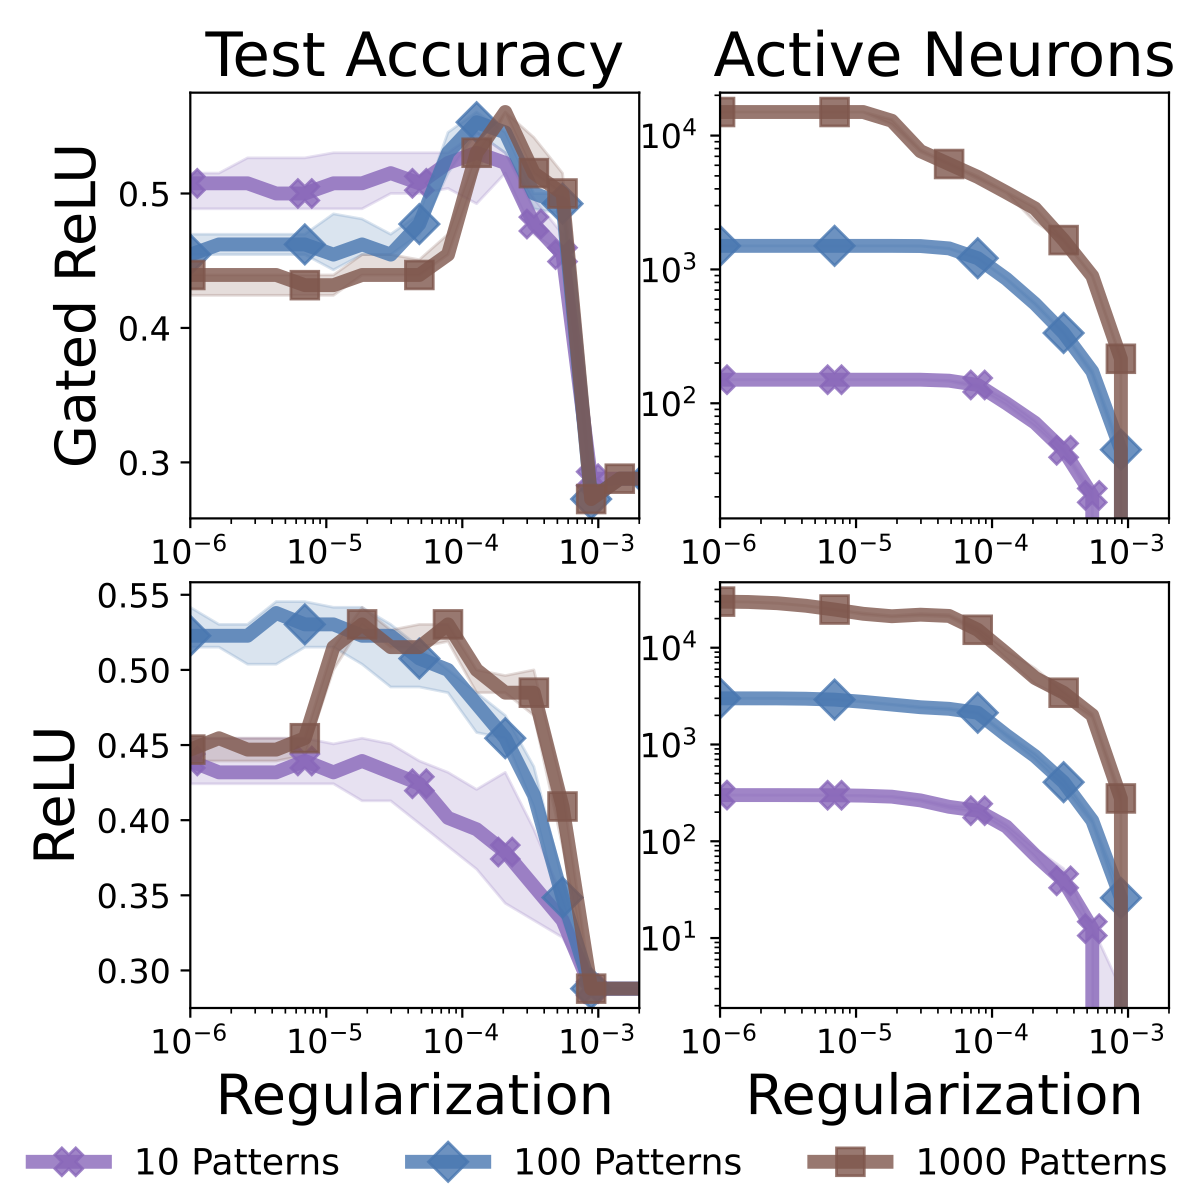
\includegraphics[width=0.6\textwidth]{assets/hp_paper.png}
%    \end{figure}
%    \begin{itemize}
%        \item Variance induced by resampling \( \tilde \calD \) is minimal.
%        \item Standard bias-variance trade-off.
%    \end{itemize}
%\end{frame}

%\begin{frame}{Bonus: Sub-sampling Patterns Cont.}
%    \begin{table}[t]
	\centering
	\begin{small}
		\begin{tabular}{lccc} \toprule
			\textbf{Dataset} & \textbf{Convex} & \textbf{Adam} & \textbf{SGD}  \\ \midrule
			magic            & 85.9            & \textbf{86.9} & 86.4          \\
			statlog-heart    & \textbf{83.3}   & \textbf{83.3} & 79.6          \\
			mushroom         & \textbf{100}    & \textbf{100}  & 99.9          \\
            vertebral-col.   & \textbf{90.3}    & \textbf{90.3} & 88.7          \\
			cardiotocogr.    & \textbf{89.9}   & 36.5          & 88.9          \\
			abalone          & \textbf{66.2}   & 65.3          & 66.1          \\
			annealing        & 90.6            & \textbf{93.7} & 88.7          \\
			car              & 87.8            & \textbf{94.8} & 90.1          \\
			bank             & 89.8            & \textbf{90.8} & 90.5          \\
			breast-cancer    & \textbf{68.4}   & 64.9          & \textbf{68.4} \\
			page-blocks      & 94.0            & \textbf{97.1} & 96.9          \\
			contrac          & \textbf{55.1}   & 54.4          & 53.7          \\
			congressional    & 63.2            & 62.1          & \textbf{67.8} \\
			spambase         & 93.3            & \textbf{93.5} & 93.2          \\
			synthetic        & \textbf{98.3}   & 96.7          & 96.7          \\
			hill-valley      & \textbf{65.3}   & 62.8          & 55.4          \\ \bottomrule
		\end{tabular}
	\end{small}
\end{table}

%\end{frame}

%\begin{frame}{Bonus: Sub-Optimal Pruning}
%    \begin{algorithm}[H]
%        \caption{Pruning solutions}
%        \begin{algorithmic}
%            \STATE {\bfseries Input:} data matrix \( X \), solution \( \theta \).
%            \STATE \( k \gets 0 \).
%            \STATE \( \theta^k \gets \theta \).
%            \WHILE {\( \exists \beta \neq 0 \) s.t. \( \sum_{\bi \in \act(\theta^k)} \beta_\bi D_i X \theta_i^k = 0 \)}
%            \STATE \( \bi^k \gets \argmax_{\bi} \cbr{|\beta_\bi| : \bi \in \act(\theta^k)}  \)
%            \STATE \( t^k \gets 1/|\beta_{\bi^k}| \)
%            \STATE \( \theta^{k+1} \gets \theta^k (1 - t^k \beta_\bi) \)
%            \STATE \( k \gets k + 1 \)
%            \ENDWHILE
%            \STATE {\bfseries Output:} final weights \( \theta^k \)
%        \end{algorithmic}
%    \end{algorithm}

%\end{frame}

%\begin{frame}{Bonus: Sub-Optimal Pruning}

%    \begin{algorithm}[H]
%        \caption{Pruning solutions}
%        \begin{algorithmic}
%            \STATE {\bfseries Input:} data matrix \( X \), solution \( \theta \).
%            \STATE \( k \gets 0 \).
%            \STATE \( \theta^k \gets \theta \).
%            \WHILE {\( \exists \beta \neq 0 \) s.t. \( \bad{\sum_{\bi \in \act(\theta^k)} \beta_\bi D_i X \theta_i^k = 0} \)}
%            \STATE \( \bi^k \gets \argmax_{\bi} \cbr{|\beta_\bi| : \bi \in \act(\theta^k)}  \)
%            \STATE \( t^k \gets 1/|\beta_{\bi^k}| \)
%            \STATE \( \theta^{k+1} \gets \theta^k (1 - t^k \beta_\bi) \)
%            \STATE \( k \gets k + 1 \)
%            \ENDWHILE
%            \STATE {\bfseries Output:} final weights \( \theta^k \)
%        \end{algorithmic}
%    \end{algorithm}

%    \pause
%    Approximate with least-squares fit:
%    \[
%        \hat{\beta} \in \argmin_{\beta} \half \norm{\sum_{\bi \in \act(\theta^k) \setminus j} \beta_\bi D_i X \theta_i^k - D_j X \theta_j}_2^2
%    \]
%\end{frame}

%\begin{frame}{Bonus: Sub-optimal Pruning}
%    Approximate with least-squares fit:
%    \[
%        \hat \beta \in \argmin_{\beta} \half \norm{\sum_{\bi \in \act(\theta^k) \setminus j} \beta_\bi D_i X \theta_i^k - D_j X \theta_j}_2^2
%    \]

%    \horizontalrule

%    \begin{itemize}
%        \item Algorithm is just structured pruning with a \good{correction step}!
%              \pause
%        \item We use \good{existing literature} for structured pruning to select \( j \).
%              \pause
%        \item \bad{Brute-force search} works best:
%              \[
%                  \argmin_{j} \cbr{\min_{\beta} \half \norm{\sum_{\bi \in \act(\theta^k) \setminus j} \beta_\bi D_i X \theta_i^k - D_j X \theta_j}_2^2}
%              \]
%    \end{itemize}

%\end{frame}

%\begin{frame}{Bonus: Complexity of Pruning}

%    \begin{algorithm}[H]
%        \caption{Pruning solutions}
%        \begin{algorithmic}
%            \STATE {\bfseries Input:} data matrix \( X \), solution \( \theta \).
%            \STATE \( k \gets 0 \), \( \theta^k \gets \theta \).
%            \WHILE {\( \exists \beta \neq 0 \) s.t. \( \sum_{\bi \in \act(\theta^k)} \beta_\bi D_i X \theta_i^k = 0 \)}
%            \STATE \( \vdots \)
%            \ENDWHILE
%            \STATE {\bfseries Output:} final weights \( \theta^k \)
%        \end{algorithmic}
%    \end{algorithm}


%    \begin{itemize}
%        \item Computing \( a_i = D_i X \theta_i^0 \) for every neuron: \( O(ndp)  \)
%              \pause
%              \vspace{1ex}
%        \item Checking for linear dependence: at most \( 2p \) times, do
%              \pause
%              \vspace{1ex}
%              \begin{itemize}
%                  \item check (at most) \( n+1 \) \( a_i \) vectors for linearly dependence.
%                        \pause
%                  \item Form matrix \( A \) and take SVD to compute null space: \( O(n^3) \).
%                        \pause
%                  \item Prune neuron: update at most \( n \) weights.
%                        \pause
%                        \vspace{1ex}
%              \end{itemize}
%    \end{itemize}
%    Total complexity: \( O(ndp + n^3 p) \).

%\end{frame}


%\begin{frame}{Bonus: Related Work on Convex NNs}
%    \citet{bengio2005convex, bach2017breaking} take a function space approach:

%    \begin{itemize}
%        \item Let \( \sigma \) be an activation function and define
%              \[
%                  \calH = \cbr{h : w \in \R^d, h(x) = \sigma(x^\top w)}.
%              \]
%              \pause

%        \item Write problem as optimization over function space \( W \):
%              \[
%                  \min_{w \in \calW} \cbr{\sum_{j=1}^n L\rbr{\sum_{h_i \in \calH} w_i h_i(x_j), y_j} + R(w)}.
%              \]

%              \pause

%        \item If \( R \) is sparsity inducing, then the final network may have finite width.
%    \end{itemize}

%\end{frame}


%\begin{frame}{Bonus: Related Work Cont.}
%    \citet{bengio2005convex}: algorithm-focused approach.
%    \vspace{1ex}
%    \begin{itemize}
%        \item Take \( R(w) = \norm{w}_1 \) and \( L(\hat y, y) = \max\cbr{0, 1 - \hat y y} \).
%              \pause
%              \vspace{1ex}
%        \item Show that \( \text{nnz}(w^*) \leq n+1 \), meaning the final model is finite.
%              \pause
%              \vspace{1ex}
%        \item Propose a boosting-type algorithm for iteratively adding neurons.
%    \end{itemize}

%\end{frame}
%\begin{frame}{Bonus: Related Work Cont.}
%    \citet{bach2017breaking}: analysis-focused approach.

%    \begin{itemize}
%        \item Handle spaces/functions properly using measure theory.
%              \vspace{1ex}
%              \pause
%              \begin{itemize}
%                  \item \( \calW \) is a space of signed measures, prediction is
%                        \[
%                            f(x) = \int_{\calH} h(x) dw(h)
%                        \]
%                        \vspace{1ex}
%                        \pause

%                  \item \( R \) is weighted total variation of measure \( w \).
%                        \pause
%                        \vspace{1ex}

%                  \item Setup reduces to \citet{bengio2005convex} in finite spaces.
%              \end{itemize}

%              \pause
%              \vspace{1ex}
%        \item Guarantee that \( m^* \leq n \) using a representer theorem.
%              \pause
%              \vspace{1ex}

%        \item Derive an incremental algorithm based on Frank-Wolfe, but incremental steps are NP-Hard
%              for ReLU activations.
%    \end{itemize}

%\end{frame}

%\begin{frame}{Bonus: Key Representer Theorem}
%    \begin{theorem}[\citet{rogosinski1958moments}]
%        If \( \rbr{\Omega, \calB} \) is a Borel space, \( \mu \) is a measure,
%        \( g_i \), \( i \in \cbr{1, \ldots n} \) are measurable and \( \mu \)-integrable,
%        then there exists measure \( \hat \mu \) with finite support at most \( n \)
%        such that
%        \[
%            \int_\Omega g_i(\omega) d\mu(\omega) = \int_\Omega g_i(\omega) d \hat \mu(\omega)
%        \]
%        for all \( i \in \cbr{1,\ldots,n} \).
%    \end{theorem}

%    Prediction for dataset with \( n \) dimensions:
%    \[
%        f(x_i) = \int_{\calH} h(x_i) dw(h) = \sum_{h = 1}^m h_j(x_i) w(h_j),
%    \]
%    where \( m \leq n \) and \( h_j(x) = \rbr{\abr{x, w_j}}_+ \).
%\end{frame}


\end{document}
